\documentclass[a4paper, 12pt, pdftex]{report}
\fussy
%\sloppy

% Package includes
%\usepackage{setspace}
% \onehalfspacing
% \usepackage[margin={1in, 1in}]{geometry}
\usepackage{natbib}
\bibpunct[: ]{(}{)}{;}{a}{,}{,}
\usepackage{graphicx}
%\usepackage{amssymb}
\usepackage{color}
\usepackage{subfigure}
\usepackage{amsmath,amssymb}
\usepackage{rotating}
\usepackage{booktabs}
\usepackage{lscape}
\usepackage[hang, bf, small]{caption}
\usepackage{hyperref}
\usepackage{listings}
\usepackage{nomencl}
\makeglossary % required by nomencl
\usepackage{makeidx}
\makeindex % required by makeidx

% \usepackage[Conny]{fncychap}
% \ChTitleVar{\centering\Huge\mdseries\sffamily}
% \ChRuleWidth{1pt}
\usepackage{fancyhdr}
\lhead{}
\usepackage[french, thinspaces]{fancynum}
\usepackage[thmmarks]{ntheorem}
\theoremstyle{plain}
%\theorembodyfont{\upshape}
\theoremsymbol{\ensuremath{\rule{0.3em}{0.3em}}}
\theoremseparator{:}
\theoremindent 1cm

%\usepackage[all]{xy}
\DeclareGraphicsExtensions{.jpg, .pdf, .mps, .png}
\graphicspath{{graph/}}

% command - typesetting in text
\newcommand\tagname[1]{{\scshape \small #1}}
\newcommand\console[1]{\ttfamily #1}
% commands - graphics
\newcommand{\fullwidth}{0.7\textwidth}
\newcommand{\halfwidth}{0.4\textwidth}

% commands - equations
\renewcommand\({\begin{equation}}
\renewcommand\){\end{equation}}
\renewcommand\deg{\ensuremath{^\circ}}

\newcommand{\eindex}[1]{\emph{#1}\index{#1}}
\newtheorem{example}{Example}[chapter]
\newenvironment{overview}{\begin{quote}}{\end{quote}}

% Title and author definitions
\newcommand\thetitle{Process Control Laboratory Handbook}
\title{\thetitle}
\newcommand\theauthor{Lourens du Plessis and Carl Sandrock}

\begin{document}

% First title page
\begin{titlepage}
  \begin{center}%
    
\includegraphics[width=\textwidth]{pmclogo}
    \vfil
    {\huge\scshape \thetitle \par}%
    \vskip 3em%
    {\large
       \theauthor
      %  \vskip 1.5em%
      % {\large \today \par}%       % Set date in \large size.
    }
  \end{center}\par
  \vfil\null
\end{titlepage} 

% Page numbering: Off
\pagestyle{empty}
\thispagestyle{empty}

\tableofcontents
\listoffigures
\listoftables
\printnomenclature % The orginal command was \printglossary Later versions of miktex require the present command


% \include{matlab}
\pagestyle{headings}

\chapter{Introduction}

\section{Process control laborotory}
The process control laborotory (`The Lab') exists to provide the process control student the opportunity to get their hands dirty and apply theoretical knowledge gained in the classroom to a practical problem.  From the real control valves and measuring equipment to the top-class A/D conversion and historian system, from the hands-on building of equipment to the programming of complex controllers in a simulated environment, the lab gives many oppertunities for exploration.

\section{This manual}
There are many possibilities to explore in the lab but such diversity and scope brings about confusion if not properly mapped out.  This manual represents a collection of the experience of many students.  It is an organic document, which grows with each successful project, whether it is stricty academic or not.  The contents of the manual include, but are not limited to the running of the rigs, settings on the computers and the general hints.  Use it wisely and add to it to let it grow.
%\chapter{Introduction}
The document gives an overview of the different components associated with the implementation of a data acquisition and control system, to enable the control of the experimental setups with the use of the computer. This was achieved through the centralised implementation of an analog to digital (A/D) and digital to analog (D/A) conversion instrumentation called the OPTO22 SNAP I/O range.

Certain protocols or methods were accordingly defined to standardise the implementation of the physical wiring and the software used, and this document discusses these methods. Some practical issues surrounding the implementation an control system on an experimental setup is also discussed. 

The document is divided into the following chapters:
\begin{description}
	\item [Chapter 2] gives an overview of the different issues surrounding the measurement and control of a ``real'' process.
	\item [Chapter 3] discusses the different software components, and their interaction, used in the acquisition of the data and the control of the different experimental setups.
	\item [Chapter 4] defines the protocols and methods used for the analog wiring of the instrumentation.
	\item [Chapter 5] discuss the different documentation types used in documenting the data acquisition and control system as well as the data base that was developed to store the relevant information.
\end{description}
\chapter{Measuring and control devices}
\begin{overview}
The different issues surrounding the measurement and implementation of an analog control system is discussed. This includes the filtering of noise, the analysis of instrument error and a generic procedure for the calibration of the instrument. 

A theoretical discussion on cold junction compensation  for thermocouple measurement is also given.  
\end{overview}

\section{Noise and filtering}
\eindex{Noise} is characterised by high frequency disturbances with a zero net effect on the measurement and arises from a number of sources such as \citep[538]{Seborg89}:
\begin{enumerate}
	\item the measuring device,
	\item electrical equipment such as a.c. power circuits, generators and turbines, 
	\item that inherently part of the process (i.e. boiling liquid level measurement).
\end{enumerate}
The \emph{noise} generated by these sources degrades the signal condition that is used for the control of the process. This will cause a decrease in controller performance, especially for controllers that use an approximation of the derivative error. The \emph{noise} can however be removed from the incoming signal as it contains no valuable information \citep[389]{Marlin00} for control. Noise is mainly reduced by using proper shielding and grounding or \emph{filtering}. 

Two types of filters can be identified \citep[539]{Richardson94} and are \eindex{analog filters} or \eindex{digital filters}. The \emph{analog filters} are implemented as electrical networks and is used to \eindex{condition} (i.e. to remove or minimize the noise) continuous signals. \emph{Digital filters} are implemented as software on the computer and \emph{condition} sampled data signals \citep[539]{Richardson94}. The theory on which both filters are based, are the same although the implementation may differ.

The filter calculation usually employed in the chemical processing industry is a first order lag or \eindex{low pass filter} \citep[390]{Marlin00}. Its operation can be described by an differential equation of the form:
\(\tau_f\frac{dy(t)}{dt} + y(t) = x(t) \)
with $x(t)$ the data to be filtered, $y(t)$ the raw measurement and $\tau_f$ the filter time constant. The equivalent transfer function description is:
\begin{align}
	x(s) &=  \tau_f y(s)s + y(s)  \nonumber \\
	\therefore \quad y(s) &= \frac{1}{\tau_f s + 1}x(s)
\end{align}
The gain of the filter is one as the filter must not influence the measurement other than reducing the high frequency noise. 
	
The discrete implementation of the filter can be derived and is known as an \eindex{exponential filter} \citep[539]{Seborg89}:
\begin{align}
	x_n &= \tau_f \frac{y_n - y_{n-1}}{\Delta t} + y_n  \nonumber \\
	\therefore \quad y_n &= \frac{\Delta t}{\tau_f + \Delta t}x_n + \frac{\tau_f}{\tau_f + \Delta t}y_{n-1}
\end{align}
The general exponential filter can be written by defining:
\(1 - \alpha \stackrel{\Delta}{=} \frac{\tau_f}{\tau_f + \Delta t} \)
to give,
\(y_n = \alpha x_n + (1 - \alpha)y_{n-1} \)

A frequency plot (Bode plot) of the \emph{low pass filter} shows (figure~\ref{fig:digi:digifilter}) how the fact that the magnitude drops rapidly can be used to reduce the effects of noise by ensuring that the filter gain is small at the frequencies where noise is encountered. 

The filter time constant is used to determine the magnitude at the specified frequency. The filter time constant can, for example, be increased to filter lower frequency noise.
	\begin{figure}[htbp]
		\centering
		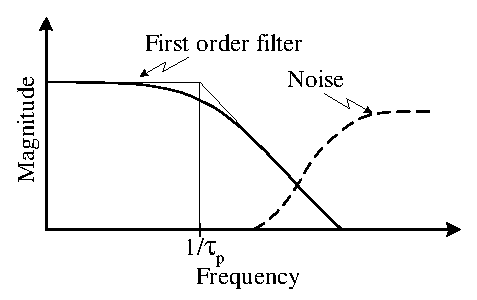
\includegraphics[width = 0.6\textwidth]{digifilter}
		\caption{Low pass filter}
		\label{fig:digi:digifilter}
	\end{figure} 
	
\begin{example}
	A sinusoidal noise measurement with a frequency of 10 rad/s and amplitude of 0.1 is shown in figure 						\ref{fig:digi:boderaw}. A low pass filter can therefore be designed to reduce this noise.
	\begin{figure}[htbp]
		\centering
		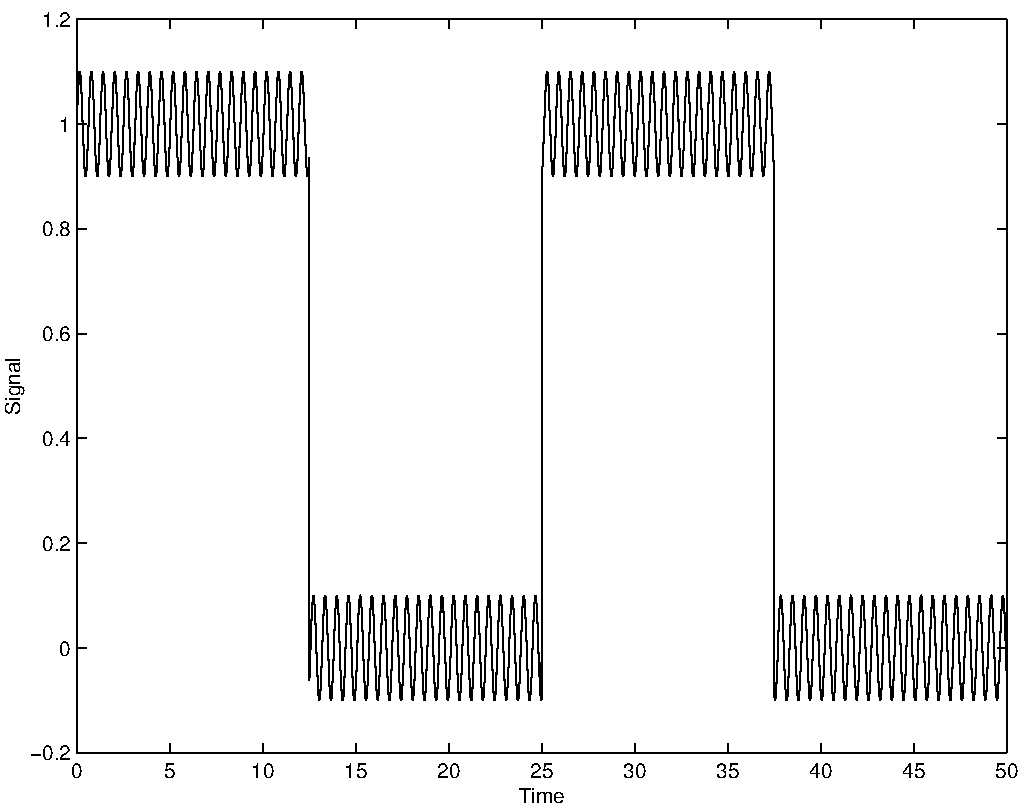
\includegraphics[width = 0.6\textwidth]{digiboderaw}
		\caption{Raw measurement data}
		\label{fig:digi:boderaw}
	\end{figure}
	
	A filter that will reduce the noise by 80\% is developed by firstly specifying the filter gain ($G_f$): 
	\[ \frac{x(s) - y(s)}{x(s)} = 0.8 \]
	\[\therefore \quad G_f = \frac{y(s)}{x(s)} = 0.2\]
	and secondly determine the filter time constant ($\tau_f$), using the magnitude frequency response of the filter transfer function:
	\[G_f = \frac{1}{\sqrt{1 + \omega^2 \tau^2}}\]
	\[\therefore \quad \tau_f = \frac{\sqrt{(\frac{1}{G_f})^2 - 1}}{\omega} = \frac{\sqrt{(\frac{1}{0.2})^2 - 				1}}{10} = 0.5 \]
	to give the low pass filter:
		\[G_{f} = \frac{1}{0.5s + 1} \]
	
	The filter can accordingly be placed in series with the measured data to condition the signal and the 					resultant output signal can be seen in figure~\ref{fig:digi:bodefilter}. 
	\begin{figure}[htbp]
		\centering
		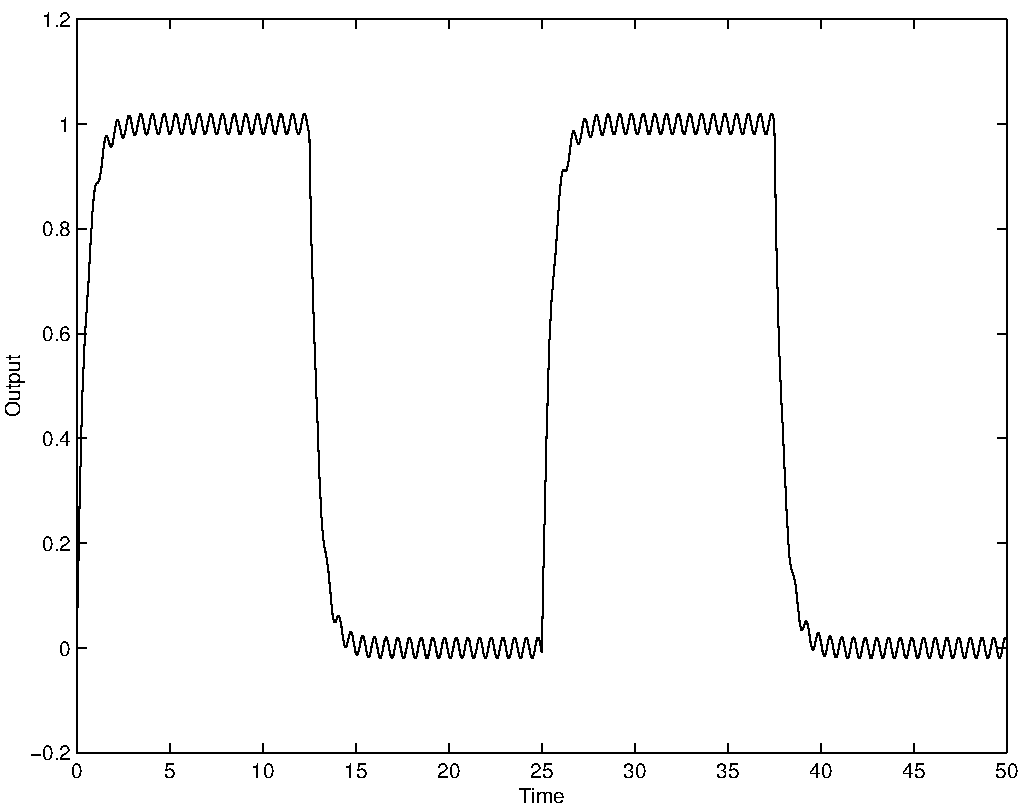
\includegraphics[width = 0.6\textwidth]{digibodefilter}
		\caption{Filtered data}
		\label{fig:digi:bodefilter}
	\end{figure}
	It can be noted that the filter will, however, slow the response of the signal measurement and is slowed more 	as the signal is filtered more. The degradation of the measured signal due to noise and that due to the 				implementation 	of the filter must therefore be optimised. 
	
	Signals used for compressor surge control will, for example, not be filtered as rapid large changes can occur 	that needs immediate action, while level measurement of a storage tank can be filtered more as the process 			dynamics are slow.
\end{example}   

\section{Sensor and actuator calibration}
A sensor or actuator is usually calibrated by adjusting the low range output value or \eindex{zero} as well as the \eindex{span} of the measurement or control. A generic procedure for the calibration of a measuring or control device is given, but it should be noted that the different manuals for the instrumentation should be consulted for more specific details.
\begin{description}
	\item [Step 1:]Set the measured property or the actuator to its minimum input. A tank can, for example, be emptied if a level measurement device is calibrated or a thermocouple can be placed in ice it the temperature measurement is calibrated. The minimum signal output (i.e. 4 mA or 1 VDC) is set by adjusting the ZERO setting of the instrument.
	\item [Step 2:]Set the measured property or the actuator to its maximum input (i.e. fully fill the tank for level measurement calibration) and adjust the RANGE setting to obtain the correct maximum output (i.e. 20 mA or 5 VDC).
	\item [Step 3:]Set the measured property or the actuator to half of its maximum input and check the output to see if the output is linear or non--linear.
	\item [Step 4:]Obtain a mathematical correlation for the sensor or actuator output to the measured property should Step 3 show that the measurement or actuator output is non--linear. This is done by setting the measured property or actuator at different values between the maximum and minimum values and tabulating the corresponding output values.
\end{description}

\section{Sensor and actuator characteristics}
A brief description of the more important characteristics of measurement and control instrumentation, follows. The definitions of theses characteristics is of great importance when deciding on the type of instrument to be purchased, or identifying some current control issues for the task at hand. 

\subsection{Range, span and turndown}
	\begin{description}
		\item{Range} is the region over which a quantity may be measured (input range) or transmitted (output 						range) and is defined by stating the lower and upper range values. \index{range}
 		\item [Span] is the magnitude of the range of the instrument (i.e. the difference between the upper and 					lower range values). \index{span}
		\item [Turndown] is the ratio of the upper range value to the lower range value \citep[529]{Richardson94}. 				\index{turn down}
	\end{description}	

\subsection{Sensitivity}
The \eindex{sensitivity} of a  measuring instrument or actuator is the ratio of the change in magnitude of the output signal corresponding to the change in the magnitude of the input; after a steady state has been reached\citep[529]{Richardson94}. 
\begin{example}
	Consider a typical thermocouple for which the voltage output, $E$, is given by the following expression:
    		\[E = \beta_0 + \beta_1 T + \beta_2 T^2 \]
  where T is the temperature and $\beta$ is the temperature coefficient. The sensitivity of the 									thermocouple can therefore by derived, by differentiation, to obtain:
        \[\frac{dE}{dT} = \beta_1 + 2\beta_2 T \]
  and shows that the sensitivity of this instrument is a linear function of temperature.  	
\end{example}
 
\subsection{Resolution}
\eindex{Resolution} is the minimum difference in the values of a quantity that can be discriminated by a device. Care should be taken to specify instrumentation with the correct  for the application at hand, as more sensitive equipment invariably costs more---but effective control cannot be obtained with a measurement that has a too low \emph{resolution}.

\subsection{Repeatability}
\eindex{Repeatability} gives an indication of the closeness of agreement among a number of consecutive measurements for the same value of input conditions, under the same operating conditions and approached from the same direction for the full range of the instrument \citep[530]{Richardson94}. The direction of approach must be specified as the instrument might have \eindex{hysteresis} where there is a difference in the measurement of the device for the same input condition depending on whether the measurement is increasing or decreasing (figure~\ref{fig:digi:hyst}). 				
\begin{figure}[htbp]
	\centering
	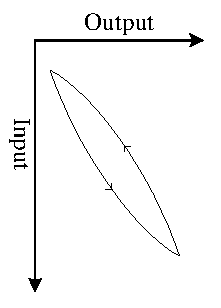
\includegraphics[width = 0.3\textwidth, angle = 90]{digihyst}
	\caption{Hysteresis of a measuring device}
	\label{fig:digi:hyst}
\end{figure}

\subsection{Measurement error}		    
\eindex{Measurement error} of an instrument is the difference between the actual measurement and the true 			value. The measurement error of instrumentation can usually be described with a Gaussian or normal 							distribution that relates the frequency of the error measurement to the measurement error 											(figure~\ref{fig:digi:standard}). 
\begin{figure}[htbp]
	\centering
	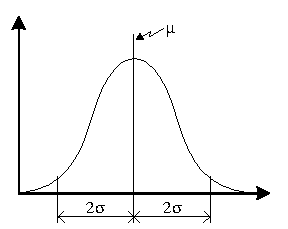
\includegraphics[width = 0.4\textwidth]{digistandard}
	\caption{Standard deviation and confidence intervals of a measuring device}
	\label{fig:digi:standard}
\end{figure}
    		
The \eindex{confidence interval} gives an indication of the maximum deviation expected for a certain 						percentage of measurements. The confidence interval usually used is $\pm$ 2 $\sigma$ from the norm and 					corresponds to 95\% of the measured data readings that is expected to lie within the defined bounds.      
\begin{example}
	The true heights and outputs are tabulated for given a sensor that is used to measure the liquid 								height in a tank. 
	\begin{table}[htbp]
		\centering
  	\caption{Liquid height measurement}
		\begin{tabular}{l c c c c c c c}
			\addlinespace[1em]
			\toprule[1pt]
				Height (cm) & 0 & 5 & 10 & 15 & 20 & 25 & 30 \\
    	\midrule[0.5pt]
    		Output (mA) & 4.1 & 6.3 & 8.9 & 12.5 & 14.5 & 17.1 & 19.8 \\
    	\bottomrule[1pt]
  	\end{tabular}
	\end{table}
The true measurement ($y$) can be calculated if it is assumed that the measured output ($y_m$) of the 					sensor should increase linearly with liquid height ($H$) over a range of 4 to 20 mA.
\begin{align}
	y &=  mH + c \nonumber\\
\therefore \quad y &= 0.53H + 4 \nonumber
\end{align}
The standard deviation ($\sigma$) can then be calculated as a function of the measured ($y_m$) and outputs ($y$), where N is the amount of measured samples \citep[25]{Johnson94}:
\begin{align}
	\sigma^2                  &= \frac{\sum{(y_{m} - y)^2}}{N-1} \nonumber\\
	\therefore \quad \sigma   &= \sqrt{\frac{0.01 + 0.12 + 0.16 + 0.3 + 0.01 + 0.02 + 0.01}{6}} \nonumber\\
	\therefore \quad \sigma   &= 0.33 \nonumber
\end{align}
If it is assumed that the measurement error can be described with a Gaussian distribution, as is the case 			for most measurements, the measurement error can be presented by $y_{m}\pm 2\sigma = y_{m}\pm 0.7 mA$ for 			a 95\% confidence interval. This corresponds to a  3.5\% error margin in the measured output. 
\end{example}

\subsection{Dead band}		
\eindex{Dead band} is the range over which the input to the instrument can be varied without the responding to the output. This a characteristic of control valves that are ``sticking''. A typical response curve for an instrument that has \emph{dead band} can be seen in figure~\ref{fig:digi:dead}.
\begin{figure}[htbp]
	\centering
	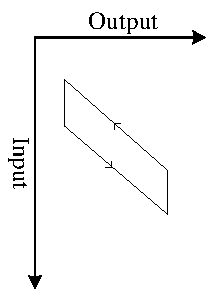
\includegraphics[width = 0.3\textwidth, angle = 90]{digidead}
	\caption{Dead band  response of a measuring device}
	\label{fig:digi:dead}
\end{figure}        

%\section{Measurement descriptions}
%The devices is responsible for the measurement of different properties of the process. This information can be used to infer the control
%actions that must be taken. The measurement usually contains two parts, viz. a \eindex{sensor} and a \eindex{transmitter}
%\citep[200]{Seborg89}. The \emph{sensor} converts the measured property into a useful electrical signal while the \emph{transmitter} will: 
%\begin{itemize}
%	\item convert the signal to a suitable standard (4--20 mA or 1--5 VDC),
%	\item power the sensor (if needed) and,
%	\item filter the incoming signal from the sensor.
%\end{itemize}
%The two parts can be combined in one instrument, which is termed a \eindex{transducer} \citep[437]{Richardson94}, or be two different devices.
%The different types of sensor measurement is discussed further.

\section{Cold junction compensation}
\subsection{Background}
Two materials (X and Y) with different thermo-electric properties will generate a potential difference, termed a \eindex{Seebeck voltage}, if the two junctions of the materials are at different temperatures (figure~\ref{fig:digi:thermo}). This thermo-electric effect can be used to infer temperature by measuring the potential difference ($E_{XY}$). 
\begin{figure}[htbp]
	\centering
	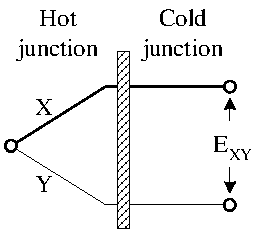
\includegraphics[width = 0.3\textwidth]{digithermo}
	\caption{Thermocouple description}
	\label{fig:digi:thermo}
\end{figure}

Five laws of thermocouple behaviour can be listed \citep[469]{Richardson94}:
\begin{enumerate}
	\item The emf depends only on the temperatures of the junctions and is independent of the temperatures of the 		wires connecting the junctions. The leads that joins the measurement (hot) and the reference (cold) 						junction may experience temperature fluctuations without effecting the reading.
	\item If a third metal Z is inserted between X and Y then, provided that the two new junctions are at the 				same temperature the emf is unchanged. A measuring device such as a voltmeter can be placed in the 							circuit without affecting the emf. 
	\item If a third metal Z is inserted between X and Y then, provided that the new junctions XY and ZY are both 		at the same temperature the emf is the same. The connections can accordingly be soldered or brazed.   
	\item If the emf obtained using the metals X and Y is $E_{XY}$ and that using metal Y and Z is $E_{YZ}$ the 			emf obtained employing X and Z will be (Law of intermediate materials):
				\(E_{XY} = E_{XY} + E_{YZ} \)
	\item If a thermocouple produces a emf $E_{XY}^{T_1 , T_2}$ when its junctions are at $T_1$ and $T_2$ 						respectively and $E_{XY}^{T_2, T_3}$ when its junctions are at $T_2$ and $T_3$ then it will produce and emf 		(Law of intermediate temperatures):
				\(E_{XY}^{T_1 , T_3} = E_{XY}^{T_1 , T_2} + E_{XY}^{T_2 , T_3}\)
		when the junctions are at $T_1$ and $T_3$. This property is used extensively for thermocouple compensation.
\end{enumerate}

\subsubsection{Thermowell}
The thermocouple must be protected against the abrasive materials that is measured. The thermocouple is subsequently placed in a \eindex{thermowell} (figure~\ref{fig:digi:thermowell}) to protect the thermocouple. It should be noted that the thermowell will influence the temperature measurement. 
\begin{figure}[htbp]
	\centering
	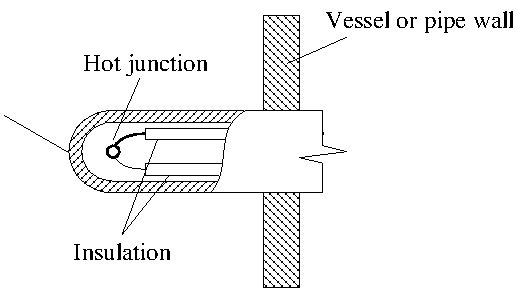
\includegraphics[width = 0.5\textwidth]{digithermowell}
	\caption{Thermocouple placed inside a thermowell}
	\label{fig:digi:thermowell}
\end{figure}

\subsubsection{Thermocouple compensation}
The thermocouple reading (emf) is a function of both the measurement ($T_1$) and reference ($T_2$) temperatures (i.e. emf = $E_{XY}^{T_1 , T_2}$). The a change in $T_2$ will therefore have an effect on the emf and will subsequently cause measurement errors. $E_{XY}^{T_1 , T_2}$ must accordingly be compensated for, by negating the effect of ($T_2$). This is accomplished through the use of the Law of intermediate
temperatures that can be written for the reference temperature:
 	\(E_{XY}^{T_1 , 0} = E_{XY}^{T_1 , T_2} + E_{XY}^{T_2 , 0}\)
where $E_{XY}^{T_2 , 0}$ varies with the reference temperature ($T_2$), that is usually another thermocouple reading (i.e. the measurement and reference temperatures are the same to give an emf = $E_{XY}^{T_2 , 0}$).

The implementation of an automatic reference junction compensator circuit can be seen in figure~\ref{fig:digi:comp}. The compensation can be implemented in the electrical circuit (i.e. reference emf is connected in series with the reading) but is inefficient if a large number of thermocouple is used as each of the readings must be compensated for on the electrical circuit. 
\begin{figure}[htbp]
	\centering
	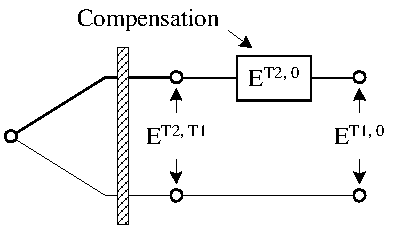
\includegraphics[width = 0.4\textwidth]{digicomp}
	\caption{Thermocouple compensation configuration}
	\label{fig:digi:comp}
\end{figure}
A more efficient configuration for a system that uses a large number of thermocouples is to do the compensation with software (i.e. the measurement emf is added to the reference emf reading).
   
%\subsection{Resistive temperature detector}
%The \eindex{resistive temperature detector} or RTD utilises the fact the resistance of a component changes with a change in temperature and can be expressed by \citep{Richardson94}:
%	\( R_x = R_0 (1 + \beta_1 T + \beta_2 T^2 + \cdots + \beta_N T^N)\)
%where $R_0$ is the resistance a 0 $^\circ{C}$ and $\beta$ are temperature coefficients of resistance.

%\subsubsection{Wheatstone bridge}
%The resistance measurement is transformed to a voltage measurement by utilising a \eindex{Wheatstone bridge}. The simplified bridge configuration can be seen in figure~\ref{fig:digi:bridge}.
%\begin{figure}[htbp]
%	\centering
%	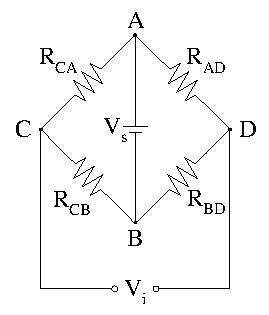
\includegraphics[width = 0.3\textwidth]{digibridge}
%	\caption{General Wheatstone bridge configuration}
%	\label{fig:digi:bridge}
%\end{figure}
%The measured voltage ($V_i$) can be given as a function of the supply voltage ($V_0$) and resistors ($R$):
%\begin{align}
%	V_{AB} &= (R_{CB} + R_{CA})I_{CB}\\
%	\mathrm{but~}\qquad I_{CB} &= \frac{V_{CB}}{R_{CB}}\\
%	\therefore \qquad V_{CB} &= V_{AB}\frac{R_{CB}}{(R_{CA} + R_{CB})}    
%\end{align}
%It can also be shown by the same calculation that:
%	\( V_{BD} = V_{AB}\frac{R_{BD}}{(R_{AD} + R_{BD})}\)
%But $V_i = V_{CB} - V_{AB}$ and $V_{AB} = V_s$
%	\(\therefore \qquad \frac{V_i}{V_s} = \frac{R_{CB}}{(R_{CA} + R_{CB})} - \frac{R_{BD}} {(R_{AD} + R_{BD})} \label{eq:digi:bridge}\) 
%Equation~\ref{eq:digi:bridge} shows that a change in resistances $R_{CA}$ and $R_{CB}$ will have an influence on the measured voltage
%($V_i$). 

%The bridge configuration is said to be balanced when the measured potential difference is zero (i.e. $V_{CB} = V_{AB}$). The different relationships for the resistors used can accordingly be written as:
%\begin{align}
%	\frac{R_{CB}}{(R_{CB} + R_{CA})} &= \frac{R_{BD}}{(R_{BD} + R_{AD})} \\
%	\therefore R_{CB} &=	R_{CA}\frac{R_{BD}}{R_{AD}} 
%\end{align}
%The bridge can therefore be balanced by adjusting $R_{CB}$ is the other resistances are known.
            
%\subsubsection{Three wire implementation}
%Figure~\ref{fig:digi:rtd} shows the typical three lead measuring circuit for measuring the temperature with the RTD. $R_{CA}$ and $R_{AD}$ is known, while $R_{f}$ is a variable resistance resistor that is used to balance (zero) the bridge. 
%\begin{figure}[htbp]
%	\centering
%	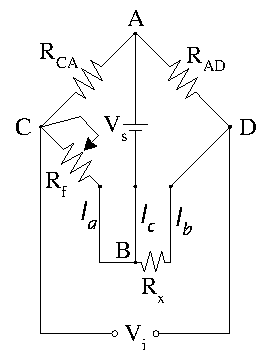
\includegraphics[width = 0.3\textwidth]{digirtd}
%	\caption{Three wire RTD configuration}
%	\label{fig:digi:rtd}
%\end{figure}

%$R_x$ is the variable resistance that changes with temperature. The ambient temperature can influence the measurement. The third wire ($l_a$) is accordingly used for temperature compensation. The circuit balances for a balanced bridge can be written:
%	\(R_{c} + R_{a} + R_{f} + R_{CA} = R_{c} + R_{b} + R_{x} + R_{AD}\)
%but, for a balanced bridge is $V_{CB} = V_{AB}$ or $R_{CA} + R_{f} = R_{AD} + R_{x}$
%	\(\therefore \qquad R_{a} = R_{b}\) 
%Any resistance effects caused by the ambient temperatures will accordingly be negated, if the two wires (a and b) have the same resistance properties ($R_a$ and $R_b$).

%\subsection{pH probe}

%\subsection{Differential pressure probe}

%\subsection{Turbine flow meter}


\chapter{Distributed control system}
\begin{overview}
The different data acquisition architectures are discussed in this chapter and the implementation of a control system using in the Simulink environment is shown. The location of the different software components are also given. 
\end{overview}

\section{Distributed data acquisition and control}
A schematic of the different \eindex{distributed control systems} that can be implemented in the process control laboratory is shown in figures~\ref{fig:control:ddcs} to ~\ref{fig:control:clust}. 
\begin{figure}[htbp]
  \centering
  \subfigure[Distributed digital control system]{
  	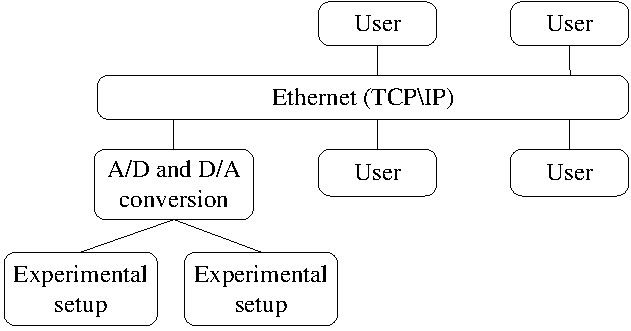
\includegraphics[width=0.6\textwidth]{controlddcs}
  	\label{fig:control:ddcs}
  }  
  \subfigure[Supervisory digital control system]{
  	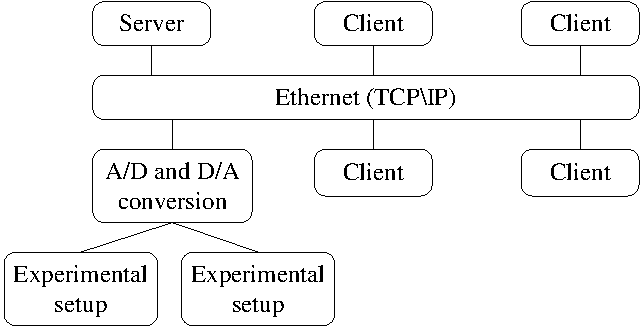
\includegraphics[width=0.6\textwidth]{controlscada}
  	\label{fig:control:scada}
  }
  \subfigure[Clustered supervisory control system]{
  	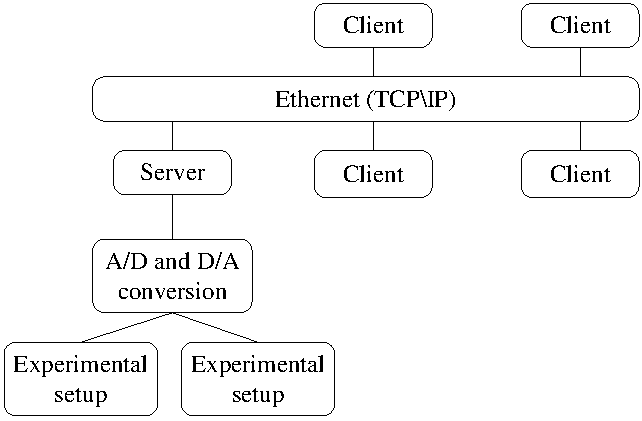
\includegraphics[width=0.6\textwidth]{controlclust}
  	\label{fig:control:clust}
  }
 	\caption{Different digital control configurations}
\end{figure}

The analog measurements is converted to a digital signal and is sent across the ethernet using the \eindex{TCP/IP} format, which is a well accepted protocol defined specifically for use with the ethernet. The control signals originating from the computers connected to the ethernet is converted back to a analog signal and sent to the actuators of the process. The different architectures regarding the interaction of the different computers on the ethernet is subsequently discussed.

\begin{description}
	\item [Distributed data acquisition and control]. The analog measurements are sent directly to the user computers through the ethernet connection and the process receives the digital control signal from the user computer via the same route. 
	
A great advantage of this approach is that any user can be used for the control of any unit should one user fail, but data integrity is at risk as there is no central data archiving device. The user computer is therefore responsible for both data acquisition and control, hence the name \eindex{distributed data acquisition and control}.   

\item[Supervisory data acquisition and control] A server is placed on the ethernet highway for the control configuration, and is responsible to give access to the different users or clients of the control system, store the data and check the  variables for alarm management. 

The fact that the clients must log onto the server before the control system can be used gives greater security and control over the different experimental setups. 

\item[Clustered supervisory data acquisition and control] The server is connected directly to the A/D and D/A instrumentation. This increases data integrity as the data to the server is not transmitted of the ethernet connection. The \eindex{bandwidth} (indication of ethernet use) of the ethernet is also reduced.
\end{description}

\section{Software and communication protocols}
The different software used (and their interaction) for the control of the experimental setups is shown in figure~\ref{fig:control:soft}. The schematic shows that there are two ways or routes to communicate with the experimental setups from Simulink, which is the software used to implement the control algorithms in the process control laboratory. 
\begin{figure}[htbp]
	\centering
	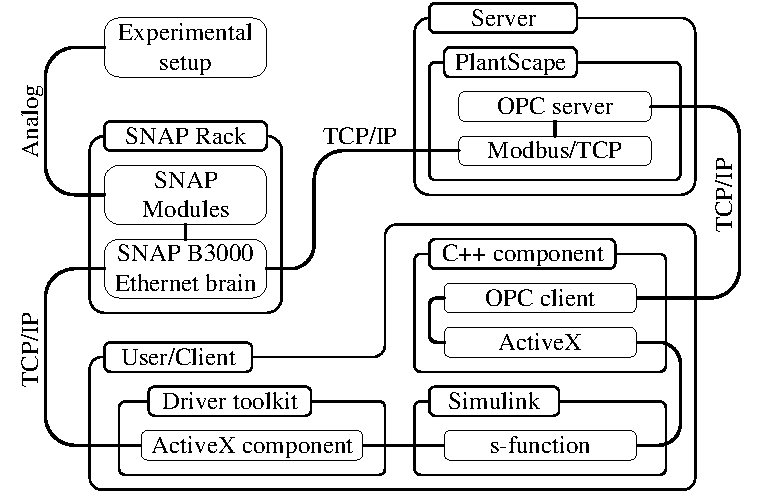
\includegraphics[width = 0.7\textwidth]{controlsoft}
	\caption{Software protocols used}
	\label{fig:control:soft}
\end{figure}

The first route can be with the use of the \eindex{driver toolkit} from OPTO22 that utilises \eindex{ActiveX}, which is a protocol defined for interfacing different software programs in the Windows environment, to communicate directly with the A/D and D/A conversion devices (SNAP B3000 brain, etc.).

The second route is with the use of a server and specific \eindex{SCADA} (Supervisory Control and Data Acquisition) software that uses \eindex{MODBUS/TCP}, a protocol defined for instrument interfacing over a ethernet connection, to communicate with the A/D and D/A conversion devices. A custom \eindex{C++ component} was developed in-house to enable \index{Simulink} that utilises \eindex{ActiveX} to communicate with the server using \eindex{OPC}, another control protocol defined for inter controller communication via ethernet connections.

Figure~\ref{fig:control:soft} shows further that the \eindex{Driver Toolkit} and the \eindex{C++ component library} must be installed on the user or client computer. The software can be found on $\backslash$$\backslash$groa$\backslash$lab$\backslash$Opto for the \eindex{Driver Toolkit} and $\backslash$$\backslash$groa$\backslash$lab$\backslash$PlantStar fot the \eindex{C++ component library}.

The s--function needed for the interfacing of \eindex{Simulink} with the experimental setups can be obtained from $\backslash$$\backslash$groa$\backslash$lab$\backslash$Rigs. More information on the development of the s--function can be obtained from the in--house \emph{Matlab Opto22 driver manual}.

The \eindex{Real time clock} block is used to force the \eindex{Simulink} simulation to run at real time and must therefore be included on the model of the control algorithm used for control. The block icon can be seen in figure~\ref{fig:control:clock}. The s--function and model of the \eindex{real time clock} can be found at $\backslash$$\backslash$groa$\backslash$lab$\backslash$Matlab$\backslash$Rtclock and must be included in the current \emph{Matlab} path to run.
\begin{figure}[htbp]
	\centering
	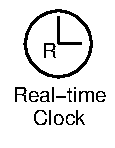
\includegraphics[width = 0.1\textwidth]{controlclock}
	\caption{Real time clock icon}
	\label{fig:control:clock}
\end{figure} 

\begin{example}
The of the s--function block using the ActiveX component \index{ActiveX component} calls for the level and flow control loop can be seen in figure~\ref{fig:control:sfunc}, and shows that two inputs for the control valves (4--20 mA) and two outputs (-20--20 mA) for the liquid level and liquid flow are available for the implementation of a control algorithm.
\begin{figure}[htbp]
	\centering
	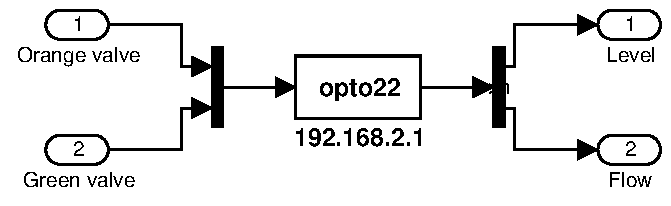
\includegraphics[width = 0.5\textwidth]{controlsfunc}
	\caption{s--function implementation of the level and flow model}
	\label{fig:control:sfunc}
\end{figure}

%An implementation of a PID controller for the tank level of the flow control loop can  be seen in figure~\ref{fig:control:model}. The one control input and the flow output is zeroed as it is not used for the current control implementation.
%\begin{figure}[htbp]
%	\centering
%	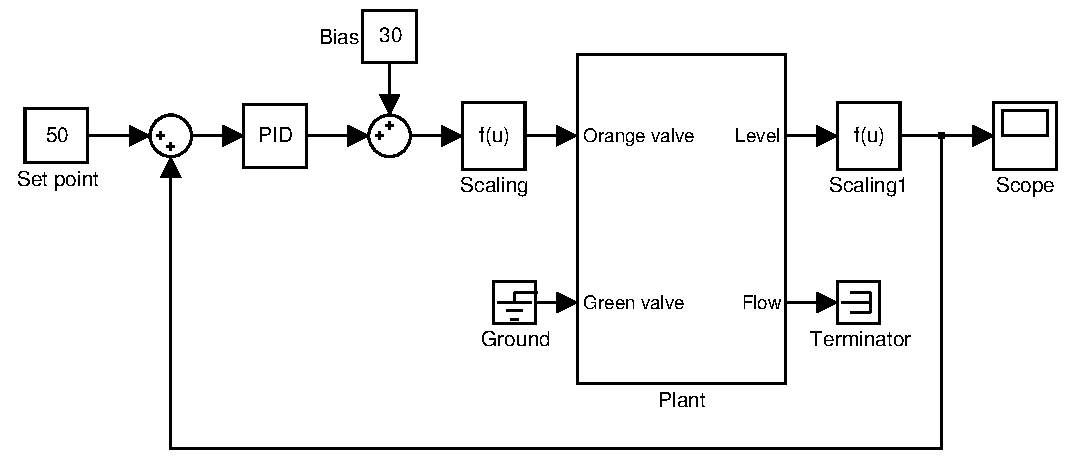
\includegraphics[width = 0.8\textwidth]{controlmodel}
%	\caption{Single loop control of the tank level}
%	\label{fig:control:model}
%\end{figure}
\end{example}
	  
\chapter{OPTO22}

\section{Introduction}
The process control laboratory has been set up with a number of experimental setups to demonstrate control principles.  These rigs are fitted with analogue process control equipment which can be used to control the processes involved.  If a computer is to be used to control the rigs, a conversion between the analogue data of the rig and the digital data of the computer must be done.  Many attempts have been made to solve this problem, with varying degrees of success.  

In addition, this approach has the disadvantage that a lot of time is spent 'reinventing the wheel' by setting up interfacing hardware and software, as well as being a less realistic image of practical control system monitoring in the field.

Interfacing with the process equipment should be less about hardware needed between the process and the computer than the actual work done on these components.  A new system removing the wiring from the process is proposed in this document, along with the requirements to be complied with to enjoy the full benefits of this system on each setup.

\section{Problem statement}
The problem of interfacing with the laboratory equipment can be broken into four parts, which will be discussed separately.  The equipment will be referred to as `rigs' and the `user' will be the person or system accessing the rigs.
\subsection{Physical interfacing}
Each element that needs to be accessed has to be physically connected to the user in some way.  The connection must be 
\begin{itemize}
	\item reliable,
	\item noise free and
	\item easily maintained.
\end{itemize}
	
\subsection{Conversion}
Conversion from analogue to digital (A/D) and from digital to analogue (D/A) signals is required.  Each experimental setup accepts analogue signals to control valves and other final control elements.  Measuring devices on the rigs return analogue data that has to be converted to digital signals for computer based control.

\subsection{Data Storage}
Data collected from the various rigs should be stored and accessible for a time period after experiments have been carried out on them.  This will enable users to do experiments without manually logging results or writing their own logging procedures.

\subsection{Software Interfacing}
All the above requirements are dedicated to providing process data and control handles to control software.  The collected and stored data must be accessible from many environments such as MATLAB and HISYS.  

\section{Conceptual design}
\subsection{General}

Conceptually, the system includes wiring to and from all the units, connected to a central bank of A/D and D/A converters connected to a central data server.  The values will be accessed using a tag system similar to SCADA systems.

The components identified above and the relationships between them are shown in Figure~\ref{fig:SCADAoverview}.

\begin{figure}
	\centering
	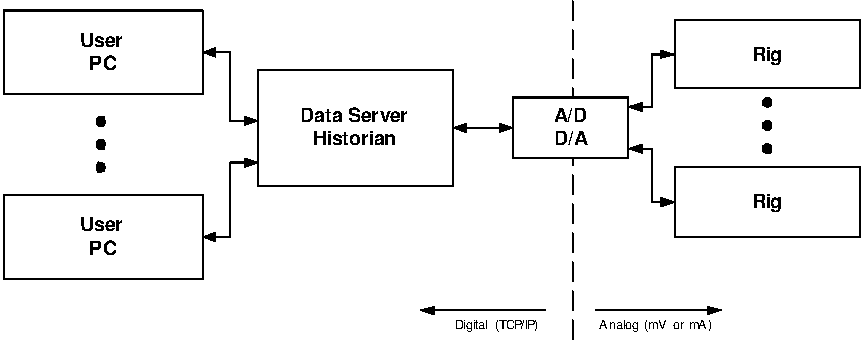
\includegraphics[width=\fullwidth]{SCADAoverview}
	\caption[Conceptual SCADA layout]{Conceptual layout of the SCADA system.  Signals to the left of the A/D-D/A line are digital, while signals to the right are analog.}
	\label{fig:SCADAoverview}
\end{figure}

It should be clear from the figure that the user does not have direct access to the analogue data, and that the server acts as an abstraction layer between the converter and the computer user.  This enables the user to focus on the design of a control system instead of worrying about the mechanics of A/D. It also protects the user from short circuits and other analogue errors on the rig.

The wiring from the experimental setup terminates in a junction box.  This junction box (JB) serves as the physical connection point between the system and the experimental setup.  It should be possible to do most of the maintenance required for each rig without ever opening the central converter's box. 

In addition to the signal interfacing, the JB should provide space for power converters as required by each rig.  This ensures that the rigs do not have high voltage power open to spills and accidental touch.

\subsection{Software interface}
The server computer will have to run software that is capable of data storage and retrieval.  Possibly a general web interface could be included.  This software should include methods to interface with the A/D converter.

\subsection{Documentation}
Documenting a complex system such as this one is challenging for the user.  A system will have to be put in place that removes most of the possibility for error.  A database system for tracking connections and changes in the rigs required.  Diagram standards for wiring and rig setups are also needed.

\section{Detail design}
\subsection{Physical interfacing}
Wiring from the central conversion unit to each of the rigs will consist of shielded single twisted pair wires.  Each wire represents a signal, using the two conductors in the wires to transfer it.  The shielding ensures that signal quality is preserved. 

Each rig is fitted with a junction box (JB), where the wiring from the central point terminates in connectors.  These connectors provide a convenient connection point for signals from the rigs, while the JB itself provides a safe environment for the open terminals and power supply units.  

Mild steel junction boxes with polycarbonate viewing windows are used.  Junction boxes are specified to IP55 standard, ensuring protection from dust and spills on the rigs.

Based on the amount of signals to and from each rig, a size of 400x300x120mm was chosen, with DIN rail mounted connectors.  Power supplies were added into the size calculations, as these should also be in the JB.

\subsection{Conversion}
The OPTO22 system will be used to handle conversion.  This system operates on an attractive modular principle, which includes conversion to and from many different analog and digital signals.  Conversion modules called SNAP modules are connected to a rack with a 'brain' unit which transfers information to the network using TCP/IP.  Information was obtained from OPTO22 (form 1112).

OPTO22 SNAP Ethernet brains are compact, flexible high performance processors for many applications.  The SNAP-B3000-ENET brain was chosen, as this is the baseline brain and complies with all the requirements while being the cheapest of the SNAP brains.  Two units are required for the signals currently used in the laboratory.

Each rack has room for 12 modules.  These may include the following convertor modules:
\begin{itemize}
	\item	AIMA-4: $\pm$20mA input (A/D)
	\item	AITM:  Thermocouple input (A/D)
	\item	AOA-23: 4-20mA output (D/A)
\end{itemize}

The OPTO22 units will be installed in a junction box of the same specifications as the rig JBs, but with the larger dimension of 800�600�210mm.  The OPTO22 housing design can be seen in Appendix A.

\subsection{Data storage and software interfacing}
Mintek has produced a SCADA-like system called PlantStar.  PlantStar, installed on a server connected to the OPTO22 box will manage data collection and retrieval.  Plantstar includes a web-based interface for monitoring and basic control.  Connections to other programs are possible using calls to the client application installed on user PCs.

The system has to be installed on a computer running Microsoft Windows 2000, with a large hard drive and more than 128MB of RAM.  A 13GB hard drive will be installed for data storage.

\subsection{Documentation}
The wiring system has many connections and tag numbers.  A systematised method is required to keep track of thes numbers.
\subsubsection{Tags}
Tag numbers conform to ISA standards.  Tags are built as follows:\bigskip

\begin{centering}
	\framebox{Rig number} -- \framebox{Object type code} -- \framebox{Object number} \bigskip \\
\end{centering}

Rig numbers are two digits padded with a leading zero if required.  Object numbers are three digits with leading zeros and increment sequentially from 001 for each unique object type on a rig.  Rig numbers and current object type codes can be found in appendix A.  These lists are dynamic, allowing for expansion of the rigs and labs.

\subsubsection{Wire names}
Wire names are generated from the numbers of the connectors the wires connect. \bigskip

\begin{centering}
\framebox{Rig connector number}  / \framebox{OPTO connector number} \bigskip \\
\end{centering}

Where both numbers are three digits padded with leading zeros.  These numbers are affixed to the wire so that they are legible when read in a direction from the rigs to the OPTO JB.

\subsubsection{Diagrams}
Three types of wiring diagrams are needed for documentation of the system:
\begin{itemize}
	\item	JB Box layout diagrams,
	\item	loop diagrams and
	\item	rig PIDs.
\end{itemize}

Diagrams for the distillation column have been drawn up and can be seen in appendix B.

\subsubsection{Equipment Database}
To simplify the documentation of the wiring and connectors, an equipment database is required.  This database tracks each piece of process control equipment and the connections between them.
The starting point for the database is the rig table, which contains the number and name of all the rigs.  From here, linked to the rig number an equipment table stores each item's type and number.  In addition, data is stored about the date of acquisition and origin of the equipment to simplify maintenance and reordering.  To make the database extendable, a table of equipment types is linked to the equipment table, storing the tag extension of the equipment type. 

Queries are defined to generate tag numbers in accordance with the standards set out above, by combining the rig number, equipment type extension and the equipment number.

In order to track connections, each equipment record also stores the unique ID of another piece of equipment.  The direction of this linked list is defined as away from the final control elements and measuring devices.  Therefore, a control valve will link to the JB connector and an OPTO snap in module will link to the OPTO JB connector.  JB connectors reference one another.  This means that the wires connecting JB connectors on both the rig and OPTO side can be traced by following the links from either side.

Wire names are generated by a SQL query, adding the numbers from the connected pieces of equipment.  A list of wire names can be drawn up in a report for wire checking.

\subsection{New equipment}
To keep the documentation current, the following steps are required when adding new equipment.

\begin{description}
\item[Step 1] Collect information
The following information is pertinent when installing new equipment:
\begin{itemize}
	\item	What type of signal does the equipment send or receive?  This will determine the module on the OPTO that the equipment will be wired to.
	\item	Are there enough connectors in the JBs to accommodate the new signal?  If not, new connectors must be installed.
	\item	Are there enough OPTO modules of the type required? If not, a new OPTO module must be installed.
\end{itemize}

\item[Step 2] Add the equipment to the equipment database.
Check that the equipment type exist by double clicking the equipment type table.  If the equipment type does not exist, add a new type on the last line of the table and close the table view.  Open the equipment table by double clicking it.  Select the rig and equipment type from the drop down list.  Enter a unique number for the equipment in the number field, then select the tag number of the equipment this item is connected to.  For instance, a thermocouple would be connected to a connector in the JB for the rig.
If there are no free connectors in the JB, follow the same steps as above for two new connectors: one in the rig JB and one in the OPTO JB.

\item[Step 3] Lay the wiring
Open the trunking and lay a new wire between the OPTO JB and the rig JB, bearing in mind that the wire must be labelled with its wire number.  Use the wire number for the wire between the connectors mentioned above.  This number is generated automatically by the database in the wire numbers query.

\item[Step 4] Connect the wires
The wires are now connected between connectors

\item[Step 5] Test
Before the equipment is used, a signal check must be run.  Using a Ohmmeter, check the resistance between the terminals of the new signal.  This should be very high.  Low values indicate a short circuit.

\item[Step 6] Connect equipment and OPTO
The wires are now connected to the equipment and to the OPTO module.
\end{description}

\section{Conclusion}
The process control laboratories have been fitted with a well designed solution to interfacing with process equipment.  Extensive document standards and the database structure that has been developed make the maintenance of the system efficient and reduces errors.  The PlantStar software used in conjunction with the OPTO22 system provides reliable centralised A/D conversion and data logging facilities.  The software also makes provision for snap in modules that can implement additional data tasks.

\section{Recommendations}
Further investigation into the OPC interface is recommended to connect more programs to the system.  Specifically, an interface to MATLAB must be developed in order for users to interface MATLAB control algorithms with their rigs.  It is also recommended that the rigs be upgraded using standard equipment in order to facilitate modular layout of rigs.

Thought should be given to the virtual connection of rigs via the data server, allowing more complex control problems to be tackled.

Software development recommended include an interface for the database which makes it more user friendly while retaining the functionality of the underlying database.  Additional methods for direct interfacing include an addin for Plantstar which will do calibration of thermocouples and pH probes.

\chapter{Analog and digital signal transmission}
\begin{overview}
The different issues surrounding the implementation of the analog wiring system in the process control laboratory is discussed. This includes the layout design of a \eindex{junction box} for each individual \eindex{experimental setup} as well as the box used to house the A/D and D/A converter instrumentation. The different protocols with regard to the different cables used in the wiring of the analog system are also given.
\end{overview}
  
\section{Signal component installation}
An overview of the analog and digital signal transmission configuration as implemented in the control laboratory can be seen in figure~\ref{fig:wire:over}. 
\begin{figure}[htbp]
	\centering
	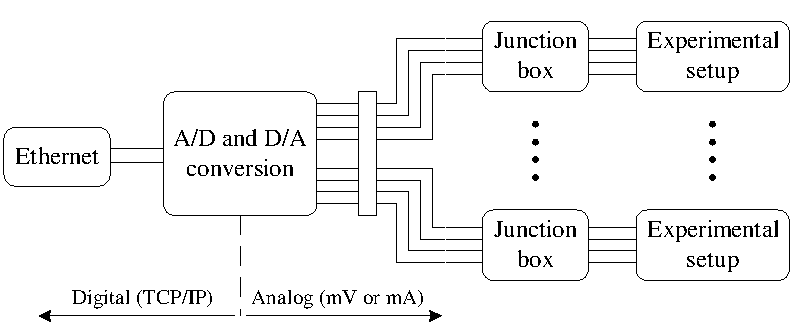
\includegraphics[width = 0.8\textwidth]{wiringover}
	\caption{Analog and digital implementation}
	\label{fig:wire:over}
\end{figure}

The analog to digital and digital to analog converters is used to transform the analog signals to a digital networking protocol called (TCP/IP) and \emph{vice versa}. All the transmission lines of the experimental setups is routed to a centralised case or box (referred to as the \eindex{Opto box}) where the A/D and D/A conversion instrumentation is situated. The box is used to protect the expensive instrumentation as well as the open connections from dust and spills and the implementation thereof can be seen in figure~\ref{fig:wire:obox}.
\begin{figure}[htbp]
	\centering
	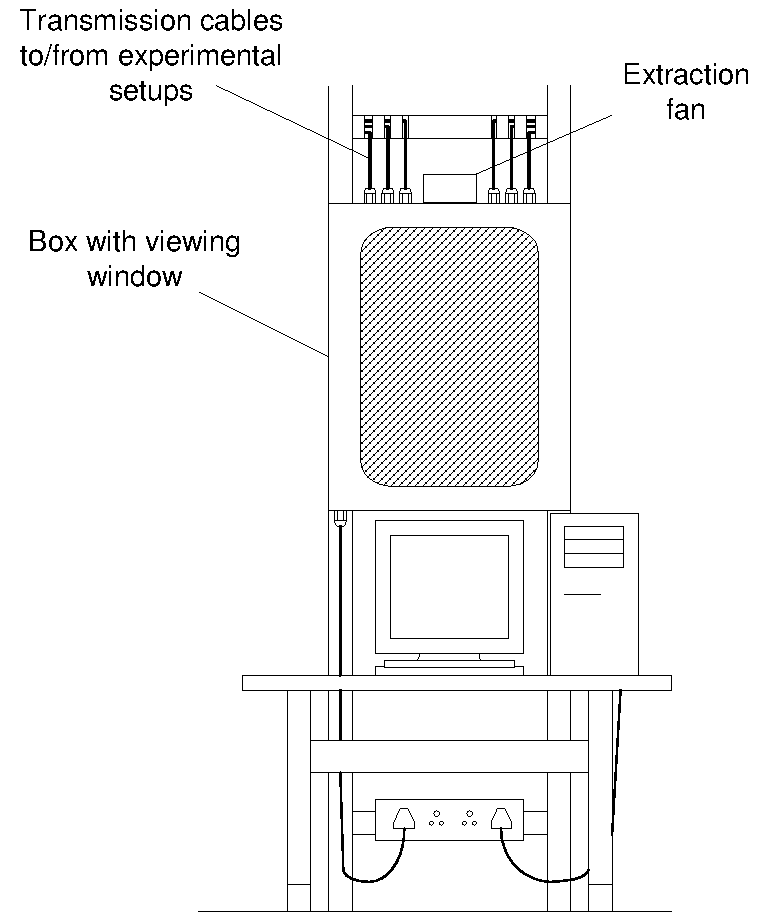
\includegraphics[width = 0.7\textwidth]{wireobox}
	\caption{Opto box installation}
	\label{fig:wire:obox}
\end{figure}

The \eindex{junction box} is inserted between the A/D and D/A converters and the instrumentation of the experimental setup and is used to:
\begin{itemize} 
	\item house the different power supplies needed for the instrumentation.
	\item create a physical connection point between the transmission lines in the trunking and that used to wire 				the experimental setup. 
	\item protect the instrumentation by inserting fuses in the transmission lines.
	\item create a save environment for the open connections and power supplies. 
\end{itemize}
The \eindex{junction box} is installed against the wall at each experimental setup together with the associated computer of the experimental setup. A graphical representation of the implementation of the \eindex{junction box} can be seen in figure~\ref{fig:wire:box}.
\begin{figure}[htbp]
	\centering
	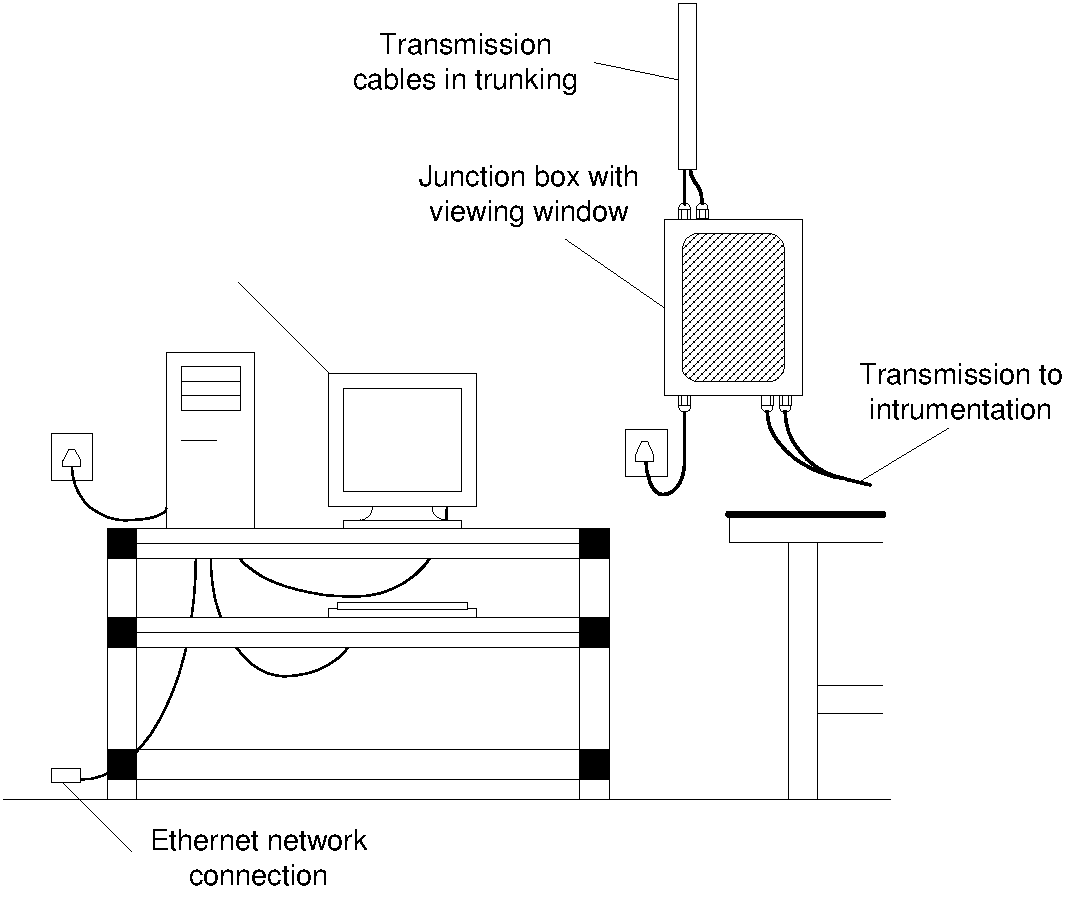
\includegraphics[width = \textwidth]{wirebox}
	\caption{Junction box installation}
	\label{fig:wire:box}
\end{figure}

The cables from the \eindex{Opto box} is situated in trunking (to keep the appearance of the process control laboratory neat) and enters the box at the top using cable glands to seal the box from dust and spills. The power cable and the cables that connects the instrumentation of the experimental setup to the junction box is separated to reduce noise contamination of the high voltage power cable on the measurement cables.

\section{Analog and digital input output instrumentation}    
The instrumentation used for the A/D and D/A conversion is the \eindex{SNAP ETHERNET I/O range} from OPTO22 and consist out of different individual components each with a specific function. A schematic of the interaction of the different components can be seen in figure~\ref{fig:wire:optoi}. 
\begin{figure}[htbp]
	\centering
	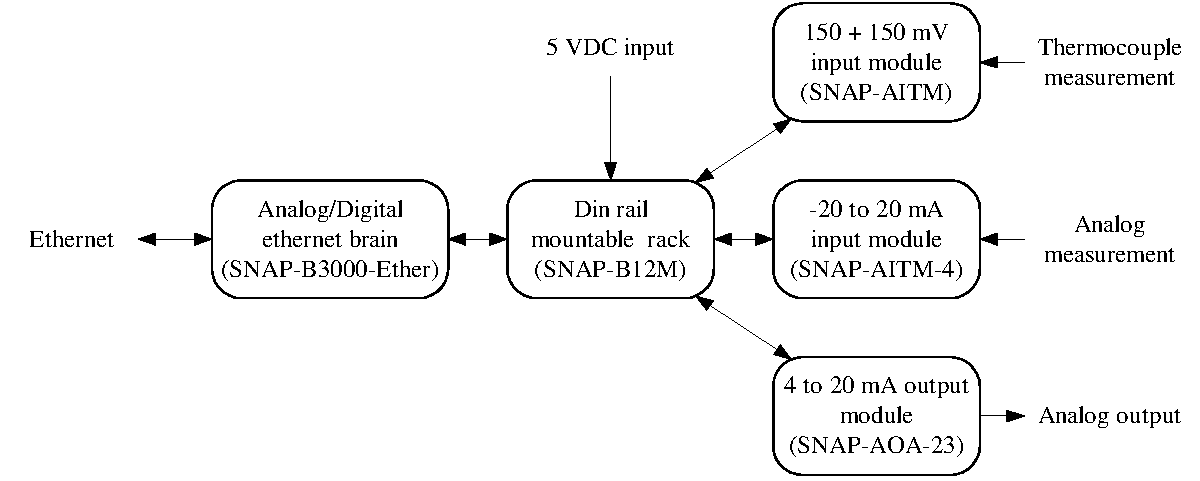
\includegraphics[width = \textwidth]{wireoptoi}
	\caption{Component specification of the SNAP I/O range}
	\label{fig:wire:optoi}
\end{figure}
Two different input modules are used for general process measurement (AITM--4) and thermocouple measurement (AIMA). One output module (AOA--23) is used for the manipulation of the actuators. The \eindex{AIMA} and \eindex{AOA--23} model has two channels while the \eindex{AITM--4} has four channels per module. The modules slot onto the \eindex{B12M rack} that is capable of housing a total of twelve modules. A breakdown of the different modules used can be seen in table~\ref{tab:wire:node} and shows that two racks are needed to house the twenty four modules
\begin{table}[htbp]
	\centering
	\caption{Module breakdown}
	\begin{tabular}{l c c}
	\toprule[1pt]
		Module name    &Channels&Modules \\
	\midrule[0.5pt] 
	  SNAP--AITM--4  &  18    &  5 \\ 
	  SNAP--AIMA     &  21		&  11\\
	  SNAP--AOA--23	 &  15    &  8 \\
	 \midrule[0.5pt]
	  Total          &  54    &  24\\
	 \bottomrule[1pt]
	\end{tabular}
	\label{tab:wire:node}
\end{table}

Every rack needs one \eindex{B3000 brain} and is used to convert the digital signal to the \eindex{TCP/IP} format, a protocol used to transfer data across the \eindex{ethernet}. The brain can be interfaced with:
\begin{description}
	\item [Modbus] which is a generic protocol devised for interfacing with third--party hardware and software. \index{Modbus} 
	\item [OPC] (object linking and embedding for control), a control protocol specifically devised for third--party software interfacing. The brain acts as an \eindex{OPC server} that can be interfaced with OPC and DDE clients.  \index{OPC} \index{DDE client} \index{OPC client}
	\item [ActiveX] (object linking and embedding for Windows) that was developed for third--party software interfacing \index{ActiveX}
	\item [HTML] that is a generic web based protocol used extensively as a communication medium on the \eindex{internet} \index{HTML} 
\end{description}

\section{Loop power}
The measuring equipment and actuators need electrical power to convert the physical properties of the process to an electrical signal that can be used for digital control and monitoring. The electricity is obtained either from the inputs used for the measurement output or as a different input supply. The use of the electrical power from the measurement signal is commonly referred to as \eindex{loop power}. 

A power supply must accordingly be used to power the signal transmission, but it is impractical to use one power supply for one measuring device. The power supply ($ES$) is therefore placed in parallel to the instruments ($XI$) requiring the power supply as can be seen in figure~\ref{fig:wire:ploop}. The A/D or D/A device ($OP$) is placed in series with the measuring instrument or actuator as it must measure or manipulate the signal. 
\begin{figure}[htbp]
	\centering
	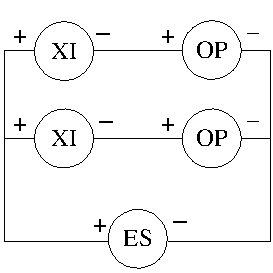
\includegraphics[width = 0.25\textwidth]{wireploop}
	\caption{Power supply implementation}
	\label{fig:wire:ploop}
\end{figure}

\section{Junction box layout}
The \eindex{junction box} is a powder painted mild steel case with a sealed hinged door with an IP55 rating (resistant to dust). A polycarbonate window was inserted into the door for illustrative purposes. A stainless steel base plate is inserted at the bottom of the box. Two C--rails are place vertically onto the base plate with bolts(see figure~\ref{fig:wire:jb}). 
\begin{figure}[p]
	\centering
	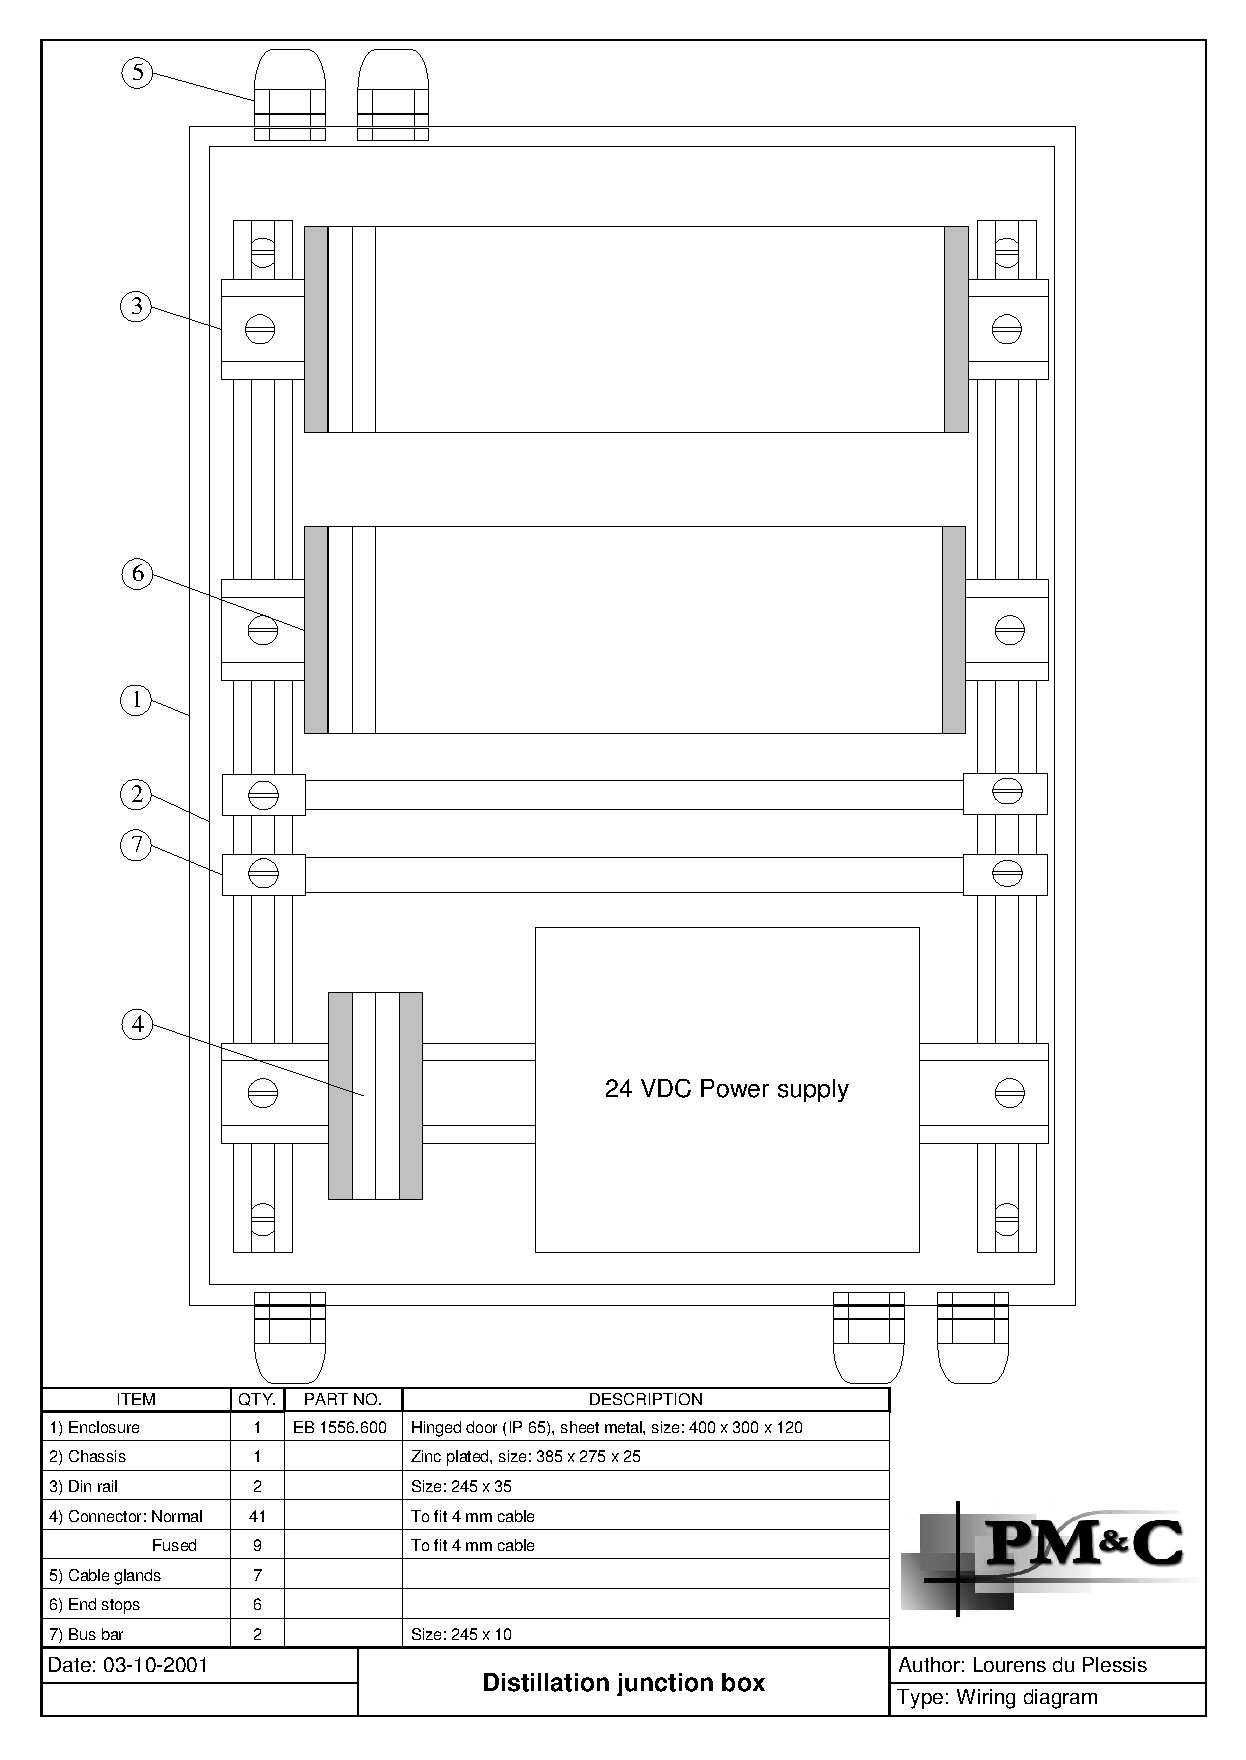
\includegraphics[width = \textwidth]{wirejb}
	\caption{Junction box layout}
	\label{fig:wire:jb}
\end{figure}

The \eindex{DIN rails} and \eindex{bus bars} are mounted onto the rails and tightened with bolts. The \emph{bus bars} and \emph{DIN rails} can therefore move freely once the bolts are loosened to give a larger degree of freedom to the box layout. The fused and normal \eindex{connectors} are specifically designed to ``clip'' onto the DIN rail and is used to connect two cables. The power supply is also placed onto the DIN rial and ensures the easy removal of the device as the base plate with all the other components need not be removed. The cables that enter the box at the top and bottom is sealed using \eindex{cable glands}. 

The \eindex{loop power} supplied by the 24V power supply is installed, in parallel with each  measuring or control loop, inside the \eindex{junction box} with the use of the \eindex{connectors} and the \eindex{bus bars}. The details can be seen in figure~\ref{fig:wire:loopp} and is based on the wiring diagram in figure~\ref{fig:wire:ploop}. 
\begin{figure}[htbp]
	\centering
	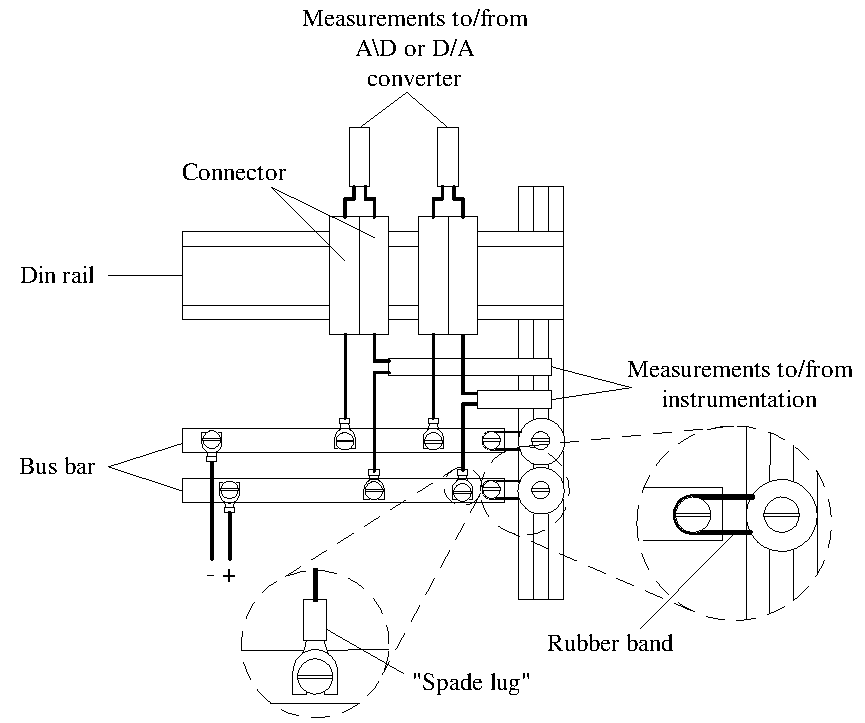
\includegraphics[width = 0.8\textwidth]{wireloopp}
	\caption{Loop power installation}
	\label{fig:wire:loopp}
\end{figure}
The \eindex{bus bar} is fixed to the C--rail by rubber bands to insulate the bar from the rest of the junction box. The cables can accordingly be fixed onto the \eindex{bus bar} with bolts and ``spade lugs''.
 
\section{Opto box layout}
The layout of the \eindex{Opto box} is based on the same principles as that of the \eindex{junction box}. The A/D and D/A instrumentation (OPTO22) are fitted to the DIN rail using custom clips and the power requirements of the instrumentation are supplied by two 5 VDC power supplies also fixed to the DIN rail.

A 220 VAC extraction fan is installed at the top of the box to remove the heat generated by the instrumentation. An air filter is installed at the bottom to act as the cool air inlet for the flow caused by the extraction fan.  
\begin{figure}[p]
	\centering
	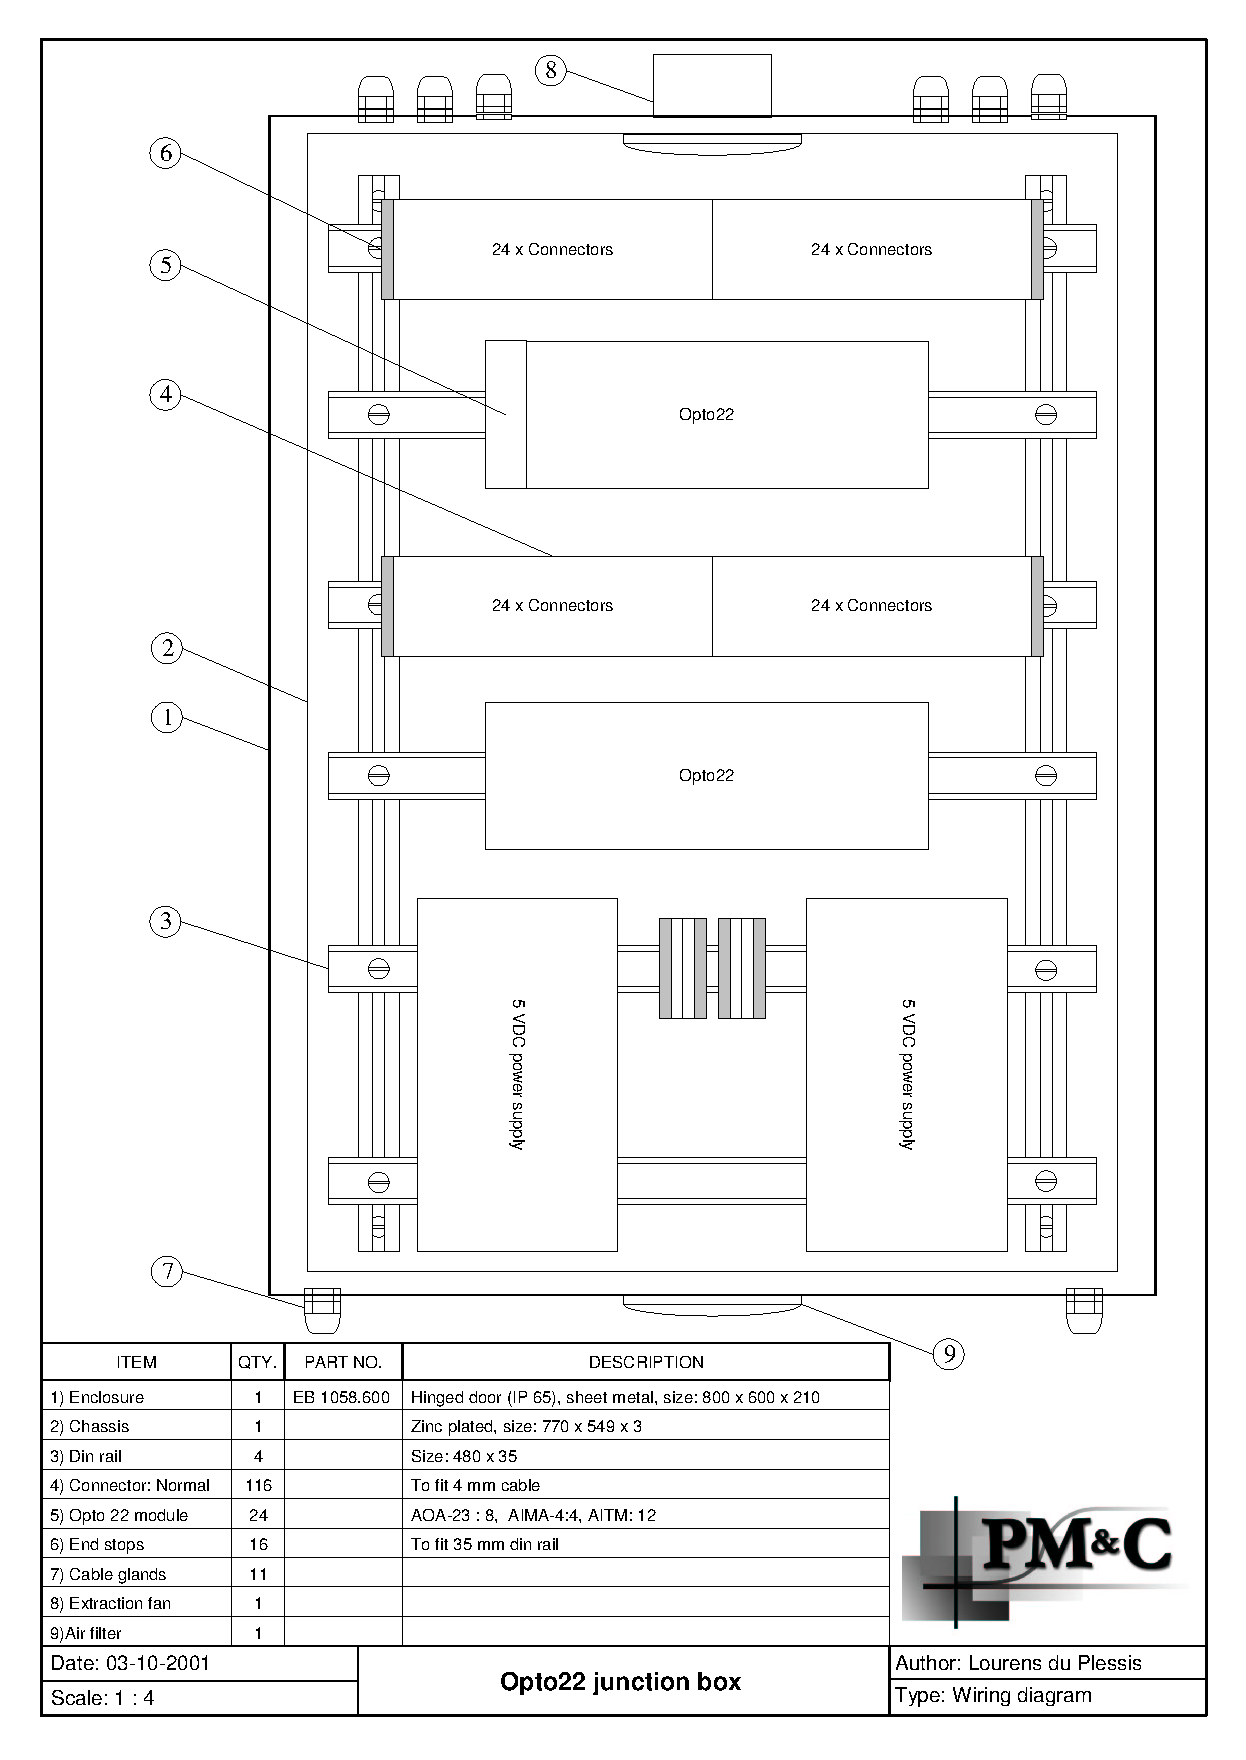
\includegraphics[width = \textwidth]{wireoptol}
	\caption{Opto box layout}
	\label{fig:wire:optol}
\end{figure}

\section{Cabling}
\subsection{Communication transmission}
The cable used for communication is \eindex{twisted pair shielded} cable with the shield placed between the outer and the inner insulation of the two individual conductors (see figure~\ref{fig:wire:comm}). This is to shield the signal in the conductors from external noise effects such as generators, heating coils, AC currents, etc. The outer insulation should be gray in colour and the two inner insulated conductors red and blue.
\begin{figure}[htbp]
	\centering
	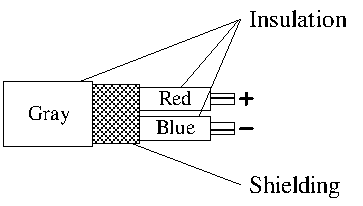
\includegraphics[width = 0.4\textwidth]{wirecomm}
	\caption{Cable used for communication}
	\label{fig:wire:comm}
\end{figure}

\subsection{Thermocouple measurement}
The cable used for the transmission of signal originating from thermocouples can be seen in figure~\ref{fig:wire:thermo}. The colour of the outer insulation is black while the inner insulation differs with the different type of thermocouple used. The colour scheme shown in figure~\ref{fig:wire:thermo} is that of a J--type thermocouple. The colour scheme for a K--type thermocouple is blue and yellow.
\begin{figure}[htbp]
	\centering
	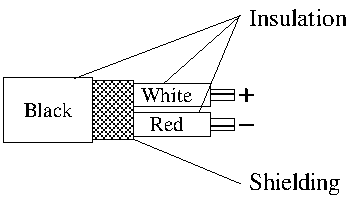
\includegraphics[width = 0.4\textwidth]{wirethermo}
	\caption{Cable used for thermocouple measurement}
	\label{fig:wire:thermo}
\end{figure}

\subsection{Power transmission}
Certain transmitters requires an extra power input. The cables used for this will therefore not be responsible for communication and must therefore be specified differently from the cable that is used for communication. The cable and colour scheme used for the purpose of power transmission for three  and two wire applications can be seen in figure~\ref{fig:wire:power} and figure~\ref{fig:wire:power2}. No shielding from electrical disturbances is needed as the cable is not used for communication. The voltages transmitted are also higher and are therefore not as susceptible to noise.
\begin{figure}[htbp]
  \centering
  \subfigure[Three wires]{
	  \hspace{3em}
  	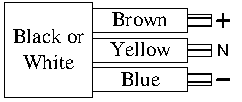
\includegraphics[width=0.3\textwidth]{wirepower}
  	\label{fig:wire:power}
	  \hspace{3em}
  }  
  \subfigure[Two wires]{
	  \hspace{3em}
  	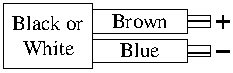
\includegraphics[width=0.3\textwidth]{wirepower2}
  	\label{fig:wire:power2}
	  \hspace{3em}
  }
 	\caption{Cable used for power transmission}
\end{figure}     

Power cables must be marked clearly with a tag stating the voltage and current type (i.e AC for alternating current or DC for direct current). This is necessary to ensure safe operation by reducing the risk of instrument damage and electrification. An example where a 220 VAC power line is marked can be seen in figure~\ref{fig:wire:mark}.
\begin{figure}[htbp]
	\centering
	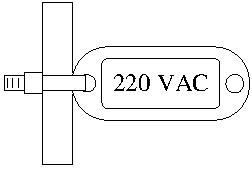
\includegraphics[width = 0.3\textwidth]{wiremark}
	\caption{Power cable marker}
	\label{fig:wire:mark}
\end{figure}

A ferrule, figure \ref{fig:digi:fer}, is placed over the exposed end points of the two conductors in the cables. This is to ensure a good (neat) connection of the cable in the connector; as the wire won't be able to bend because ferrule is rigid. 
\begin{figure}[htbp]
	\centering
	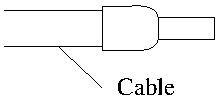
\includegraphics[width = 0.25\textwidth]{digifer}
	\caption{Ferrule placed on the end of the conductor}
	\label{fig:digi:fer}
\end{figure}    
\chapter{Rigs}
\section{General}
There are five rigs in the process control labs.  Each has unique control difficulties.  The following sections will describe how to connect MATLAB to the rigs, how each rig functions and basic procedures to follow.  The procedures described are
\begin{description}
	\item [Commissioning] This procedure is meant to be followed after the rig has been decommissioned at the end of a semester and has been standing for a period without maintenance.  During this operation, constant supervision of the rig is required to ensure that no leaks or other failures occur.
	\item [Wet startup] This procedure is to start the rig after it has been commissioned.
	\item [Shutdown] When the rig is to be used again within the near future, only a shutdown is required.
	\item [Decommissioning] When the rig is to be shelved for a significant period, a full decommissioning should be performed.  This will ensure that no extra fluids or other corrosive materials are left in the equipment and ready the rig for long-term disuse.
\end{description}

\section{The server}
One computer called the \emph{server}\index{server} in the lab is always on and connected to the network.  This computer is running Linux and is very reliable.  Information that is important to the running of the rigs that can not be found in this manual is stored centrally on the server.  Currently the server can be accessed using by navigating to \verb|groa| in windows.  Lab related information, including specific files for each rig, can be found in the directory \verb|lab|.

\section{Matlab control}
Each rig that is to be run from Matlab has a Simulink model associated with it.  These models can be found on the server.  The model will be named to reflect the rig that it represents.  To use this model, copy the model file to the directory where you will be working on the control of the rig.  From the Simulink model browser, you can open the model file and drag the model within onto a worksheet to start controlling the rigs.  These models have been set up to conform to the following standards:
\begin{itemize}\index{rig models!standards}
	\item All final control elements are activated from 0 to 1, in other words from 0\% to 100\%.  
	\item Thermocouples output temperature in \deg Celsius.
	\item Flow meters output flow in units that are specific to the rig, usually to correspond with guages on the rigs.
	\item Level meters output level in mm liquid
\end{itemize}

\section{Acetone}
The acetone flash drum control rig is currently out of commission.
\section{pH Control loop}
\subsection{Overview}
pH control is a notoriously difficult control problem not only due to its highly non-linear nature and large temperature dependence but also due to the extreme conditions experienced by measuring equipment. These problems can be investigated on the rig shown in figure~\ref{fig:rig:ph}.
\begin{figure}
	\centering
	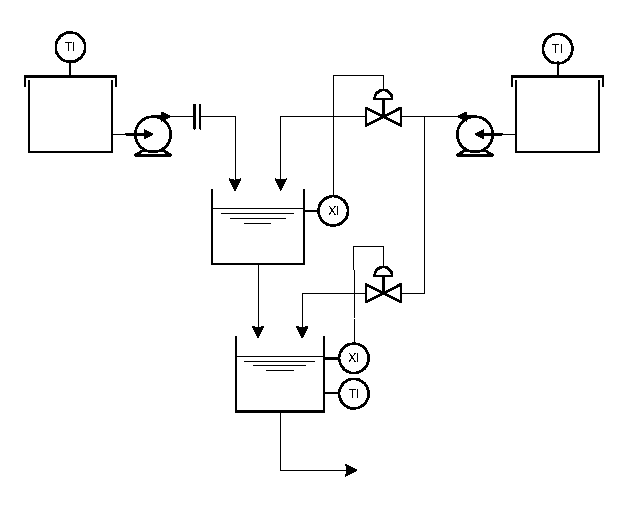
\includegraphics{pH}
	\caption{The pH control rig}
	\label{fig:rig:ph}
\end{figure}
Three temperature measurements are made to provide the possibility for temperature compensation.

\subsection{Procedures}

\subsubsection{Commissioning}

\subsubsection{Startup}

\subsubsection{Shutdown}

\subsubsection{Decommissioning}

\section{Temperature control loop with variable dead time}
The difficulties associated with the control of deadtime processes can be investigated on this rig (shown in figure~\ref{fig:rig:heat}.
\begin{figure}
	\centering
	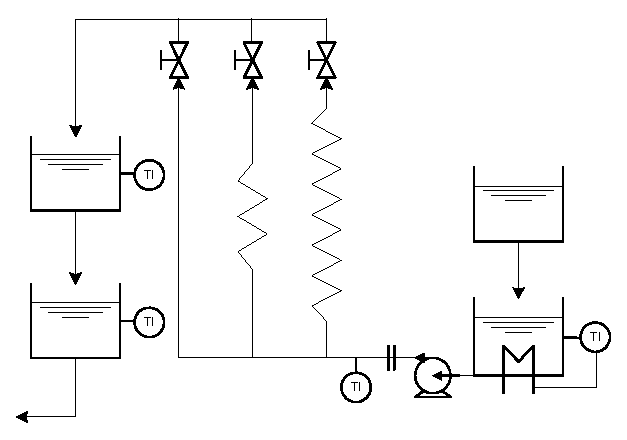
\includegraphics{Heat}
	\caption{The variable dead time temperature control rig}
	\label{fig:rig:heat}
\end{figure}
Three paths with different lengths (and different dead times) can be selected by opening and closing manual valves.  Four temperatures are measured at different points on the control loop and can be controlled by manipulating heat input from an adjustable heating element. 

\subsection{Procedures}
\subsubsection{Commissioning}
\begin{enumerate}
	\item Make a visual inspection of the equipment and ensure that no rust or obstructions are visible on the rig.  Special care should be taken to remove algal growth from the water heater.
	\item Ensure water supply is connected
	\item Ensure drain is open and unconstricted
	\item Ensure that power is supplied to the rig as well as the Thyristor
	\item Open \tagname{HV005} (Water supply valve)
	\item Ensure that water flows into the water heater
	\item Allow water level to stabilise
	\item Ensure that the float activated valve closes
	\item Follow procedure for calibrating thermocouples described in paragraph~\ref{sec:thermocouplecalibration}
\end{enumerate}

\subsubsection{Wet Startup}
This procedure is to start the rig after it has been commissioned.  There must be water in the system and the water supply must be connected with all supply valves open.
\begin{enumerate}
	\item Enable 100\% power on Thyristor
	\item Switch on mixer
	\item Ensure \tagname{HV002}, \tagname{HV003} and \tagname{HV004} are switched to the correct positions for the experiment
	\item Wait for temperature to reach setpoint temperature
	\item Switch on pump
	\item Open \tagname{HV001}
	\item Switch to automatic control on thyristor.
\end{enumerate}

\subsubsection{Shutdown}
This is the standard shutdown when the rig is still to be used in the near future.  It retains water in the rig and keeps it in readiness for a wet startup.
\begin{enumerate}
	\item Stop thyristor by pressing stop button
	\item Stop mixer
	\item Stop pump
	\item Close \tagname{HV001}
\end{enumerate}

\subsubsection{Decommissioning}
\begin{enumerate}
	\item Close \tagname{HV005}
	\item Start pump
	\item Allow tank to drain without allowing the pump to run dry
	\item Stop pump
	\item Allow water to run down from \tagname{T001} (Dead time reservoir tank)
	\item Close \tagname{HV001}
	\item Syphon off remaining water and dry tank
\end{enumerate}
\section{Level and flow control loop}

Interactive level and flow control necessitates the use of multivariable control techniques.  Figure~\ref{fig:rig:levelflow} shows the rig used for this application.  Dead time can be incorporated by using a dead time pan. 
\begin{figure}
	\centering
	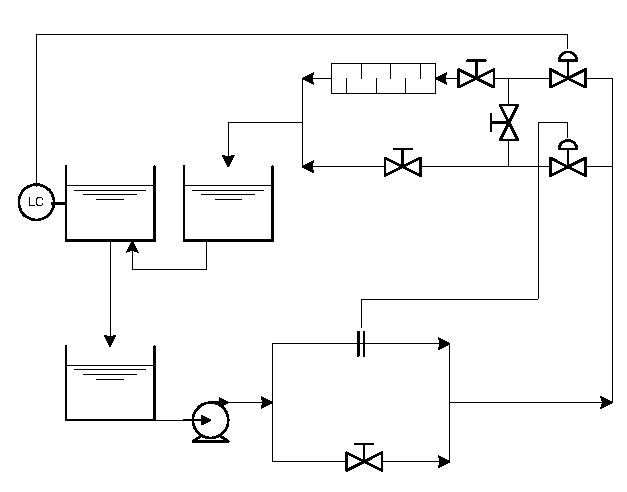
\includegraphics{LevelFlow}
	\caption{The level and flow control loop}
	\label{fig:rig:levelflow}
\end{figure}
The robust nature of the rig makes it ideal for the implementation and development of advanced analysis and control techniques like on-line tuning and fault detection.  Contemporary control techniques such as fuzzy logic or neural network control can also be attempted, as the system dynamics are straightforward and easily checked.

%\subsection{Procedures}

%\subsubsection{Commissioning}

%\subsubsection{Startup}

%\subsubsection{Shutdown}

%\subsubsection{Decommissioning}

\section{Distillation collumn control}
\subsection{Description}
The various control strategies and problems (such as inferential composition measurement) associated with distillation column control can be investigated on the rig shown in figure~\ref{fig:rig:dist}. \begin{figure}
	\centering
	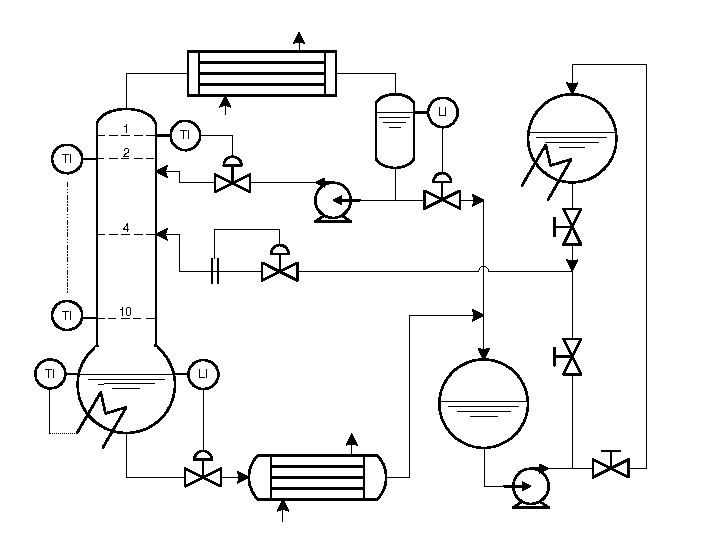
\includegraphics{Dist}
	\caption{The distillation control loop}
	\label{fig:rig:dist}
\end{figure}
Strategies that can be implemented include:
\begin{itemize}
	\item Base layer control system development
	\item Decoupling design and implementation
	\item Constrained model predictive control
	\item Temperature or composition profile control
	\item Non-linear control
	\item Automated start-up and shut down 
\end{itemize}

There are certain control problems unique to this experimental rig. The boiler-accumulator at the bottom of the distillation column is spherical. This makes the level control as well as the boil-up rate highly non-linear. Another control problem identified is that the product is mixed and recycled to the feed drum. This results in output variance being recycled back into the column.

\subsection{Procedures}
\subsubsection{Start-up}
\begin{enumerate}
	\item Open the air supply line.
	\item Adjust the pressure regulator to deliver 200 kPa.
	\item Open \tagname{05HV001} by 10\% (Small fraction).
	\item Set \tagname{05CV002} (feed valve) to 100\%.
	\item Close \tagname{05CV002} when \tagname{05LC001} (Bottoms level) is 80\%.
	\item Switch \tagname{05HS001} (thyristor power) on.
	\item Press the ``Start'' button on the thyristor.
	\item Open the cooling water supply.
	\item Set \tagname{05VC001} (thyristor) to 100\%.
	\item Set \tagname{05VC001} to desired set point when \tagname{05TI001} is more than 60 \deg C.
	\item Switch \tagname{05HS002} on (Reflux pump) when \tagname{05LC002} (Distillate level) is 50\%.
	\item Open \tagname{05CV003} (Reflux) to desired set point.
	\item Set \tagname{05CV002} to the desired set point when \tagname{05TI001} and \tagname{05TI010} stabilises.
	\item Set \tagname{05CV004} (Top) to desired set point.
	\item Set \tagname{05CV005} (Bottom) to desired set point.
\end{enumerate}

\subsubsection{Shut down}
\begin{enumerate}
	\item Close \tagname{05CV002} (Feed)
	\item Close \tagname{05CV004} (Top)
	\item Close \tagname{05CV005} (Bottom)
	\item Switch \tagname{05HS002} off (Reflux pump)
	\item Close \tagname{05CV003} (Reflux valve)
	\item Set \tagname{05VC001} (Thyristor) to 0\%
	\item Switch \tagname{05HS001} off (Thyristor power)
	\item Close the air supply line
	\item Close \tagname{05HV001} when the air pressure is zero
	\item Close the cooling water when \tagname{05TI001} is less than 60 \deg C
\end{enumerate}

\chapter{Lab Maintenance}
\section{Rigs}
\subsection{Calibration}
Measuring equipment has to be periodically recalibrated to ensure accurate operation.  New measuring equipment must also be calibrated before use.  Calibration different types of equipment is described here.  If the equipment you are attempting to use is not described here, please check documentation that was included with the equipment and update the lab manual to reflect the new equipment.

\subsubsection{Thermocouples}\index{thermocouples!calibration}\label{sec:thermocouplecalibration}
The OPTO system is capable of reading several types of thermocouples accurately.  The lab does not have a system for cold junction compensation\index{cold junction}\index{thermocouples!cold junction}, so the zero point of the thermocouples has to be measured.  This is done by immersing each thermocouple in a container filled with ice and water.  The reading of the thermocouple on the system should now be used as the compensation value.  

In Sumulink, double click on the rig block and change the compensation value for the thermocouple in question to 0 (zero).  Check the measurement from the thermocouple and enter this value into the compensation box.  The thermocouple should now read 0\deg C.

\subsubsection{pH meters}

\subsubsection{Flow meters}

\section{Computer setup}
When a new computer is brought into the lab, there are a few things that need to be done to make it work well with the other computers.  This section covers most of the custom setup that can not be done by IT personel.  Also covered are small tasks that do not justify an IT callout.

\subsection{Jobs covered by IT}
The IT services can save a lot of time when setting up a new computer or when something has happened to a computer that is not immediately fixable by anyone in the lab.  These jobs include
\begin{itemize}
	\item Network troubleshooting
	\item Periphiral setup (new network cards)
\end{itemize}

\subsection{Registering hardware}
All valuable hardware must be registered and assigned an internal reference number `Bate nommer'.  This must be done as soon as possible to avoid misunderstandings during stocktakings.  In addition to this registration, new network cards must be assigned an IP address by IT.  To do this, obtain the MAC address of the network card by either typing \verb|ipconfig| in the windows command prompt or typing \verb|ifconfig| as root on a linux machine, then call IT and tell them that you would like to register a network device.  They will ask for the MAC address and assign an IP on the DHCP server.

\subsection{PDF printer setup}

\subsubsection{Installing the printer}
Go to the Control panel, Printers section and click on Add Printer.  Select the network printer option, entering \verb|\\groa\pdfprinter| in the printer name box.  Click next.  Windows will complain about the server not having the correct drivers and will bring up a printer driver selection box.  Select a printer with colour and PostScript capabilities (the HP Colour Laserjet XXX PS works well).

\subsubsection{Setting the properties}
Before printing, right click on the printer you have just installed and select properties.  In the dialog box that follows, click the \verb|Printing preferences| button highlighted in red in figure~\ref{fig:properties}.  
\begin{figure}
	\centering
	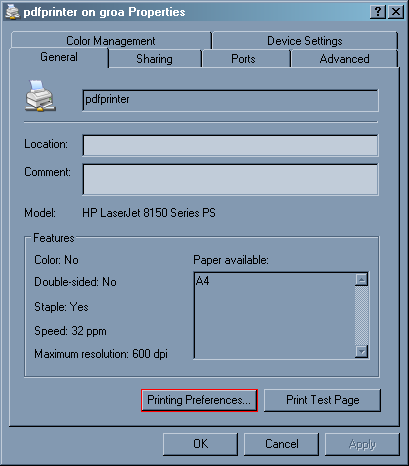
\includegraphics[scale=0.5]{properties.png}
	\caption{Printing properties dialog box}
	\label{fig:properties}
\end{figure}
Now click the \verb|Advanced| button highlighted in red in figure~\ref{fig:preferences}.  
\begin{figure}
	\centering
	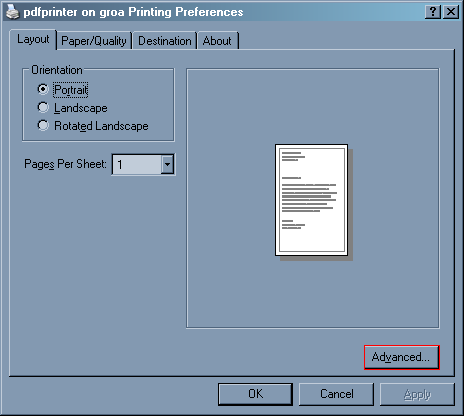
\includegraphics[scale=0.5]{preferences.png}
	\caption{Printing properties dialog box}
	\label{fig:preferences}
\end{figure}
In this advanced dialog box, make the following changes (highlighted in red on figure~\ref{fig:advanced})
\begin{figure}
	\centering
	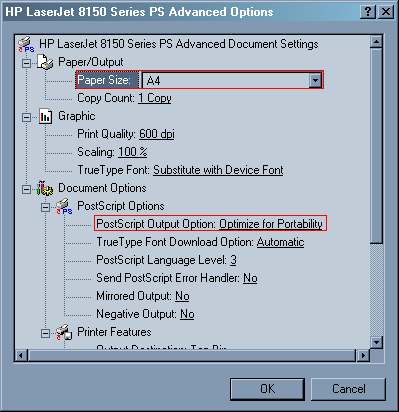
\includegraphics[scale=0.5]{advanced.png}
	\caption{Printing properties dialog box}
	\label{fig:advanced}
\end{figure}
\begin{itemize}
	\item Change the paper size to A4
	\item Click on the `Postscript Options' item in the menu to expand it and change the `Postscript output options' to `Optimize for portability'.
\end{itemize}

\subsubsection{Making a PDF}
You are now set up to make your first PDF.  Open a document in your favourite word processor and select the relevant print command\footnote{Note to Word users:  The print icon on the icon bar does not bring up a dialog box, but prints directly to the default printer -- you need to select `File/Print\dots'}.  In the dialog box that follows select the PDF printer you installed in the previous steps.  Now print normally.

\subsubsection{Getting the PDF}
The PDF will be placed in a directory shared as \verb|\\groa\PDFdrop|.  You can navigate to groa and then open this folder or you can press the windows key together with `R' and then enter the path exacly as it is typed here.  The folder will contain your PDF file with a name made up of the date and a unique job number.  Move this file to a folder on your computer and rename it to something sensible.

\section{Linux server administration}
The Linux printer server in the labs will tend to stay well-behaved most of the time.  If something does go wrong, this section will help to troubleshoot problems.  Also covered here are some basic administration commands for user maintenance
\chapter{Documentation}
\begin{overview}
Two different types of documentation as well as the corresponding ISA identification numbering used by these documents are defined for used specifically in the process control laboratory. A formal representation of the experimental setups will greatly reduce the amount of time spent on fault debugging and control loop maintenance. The two documentation types used are:
\begin{description}
	\item[Piping and instrumentation diagrams] that are used to describe piping and equipment for the different \eindex{experimental setups}.
	\item[Loop diagrams] that are used to define the wiring of the different instrumentation loops.
\end{description} 
\end{overview}

\section{Piping and instrumentation diagrams}
A \eindex{piping and instrumentation diagram} (P\&ID) is a detailed graphic representation of the process flow showing all the piping, the equipment and much of the instrumentation associated with the given process \citep[93]{Mulley93}. The different equipment and instrumentation is identified using unique numbers called \eindex{tag numbers}. The \eindex{tag number} of the different instrumentation in the process control laboratory conforms to the \eindex{ISA standards} and are defined as follows:
\begin{center}
	\framebox{Unit number} \framebox{Identifier} \framebox{Loop number}
\end{center}

The different unit numbers specified can be seen in table~\ref{tab:wire:units} while the different identifiers needed to describe the current instrumentation in the process control laboratory is listed in table table~\ref{tab:wire:ident}. The loop number is a three digit number, and is unique to each measurement loop. The sensor, transmitter and controller will therefore have the same loop number with different identifiers.
\begin{table}[htbp]
	\centering
	\caption{Unit numbers of the process control laboratory}
\begin{tabular}{ll}
\toprule[1pt]
	Number & 	Setup name \\
\midrule[0.5pt]
	01 & Acetone flashing \\
	02 & pH \\
	03 & Temperature \\
	04 & Level and flow \\
	05 & Distillation \\
	06 & OPTO22 setup \\
\bottomrule[1pt]
	\end{tabular}
	\label{tab:wire:units}
\end{table}

\begin{table}[htbp]
	\centering
	\caption{Different object types}
	\begin{tabular}{l c | l c}
		\toprule[1pt]
			Instrument  &  Identifier & Instrument& Identifier \\
		\midrule[0.5pt]
		\emph{Sensors}							 &        &                            &    \\
			Thermocouple    					 & TE     & \emph{Other} \\
			RTD					    					 & TE 		& Analog temperature controller & TC \\
			Differential pressure cell & DP 		& E/P converter							 & PY \\
			pH probe			  					 & XE 		&	Power supply               & ES \\
			Flow sensor								 & FE 		& \eindex{Junction box}      & TB \\
			Level sensor							 & LE     & \eindex{Opto box rail}     & TS \\ 
																 &        & \eindex{SNAP module}			 & OP \\													
		\emph{Transmitters} 				 &				& 													 &    \\
			Wheatstone bridge					 & TT 		& \emph{Vessels}\\
			pH transmitter						 & XT 		& Tank											 & TK \\
			Level transmitter					 & LT 		& Pump											 & CP \\
			Flow transmitter 					 & FT 	  & Heat exchanger						 & HE \\
								 								 &				& Hand valve								 & HV \\	
		\emph{Actuators}						 &				& Vapour liquid equilibrium  & VL \\
			Thyristor									 & VC \\		
			Control valve							 & CV \\
		\bottomrule[1pt]
	\end{tabular}
	\label{tab:wire:ident}
\end{table}

A list of the different symbols used in the representation of processing equipment is available in the following two references \emph{Chemical Engineering Drawing Symbols} or \emph{Control System Documentation, Applying Symbols and Identifications}. 

\begin{example}
	The tag numbering, defined from table~\ref{tab:wire:ident}, of the instrumentation and processing equipment used for a simplified pH control loop is listed in table~\ref{tab:docu:examp}.
	\begin{table}[htbp]
		\centering
		\caption{Tag number identification}
			\begin{tabular}{l l}
			\toprule[1pt]
				Instrument type & Tag number \\
			\midrule[0.5pt]
				pH sensor			  & 02XI001 \\
				pH transmitter  & 02XT001 \\
				Analog input channel & 06OP235\\
				Control valve   & 02CV001 \\
				I/P converter   & 02PY001 \\
				Analog output channel & 06OP208\\
				Tank            & 02TK001 \\
			\bottomrule[1pt]
		\end{tabular}
		\label{tab:docu:examp}
	\end{table}
	
	The P\&ID for the pH control system can accordingly be drawn using the different tag numbers of the 								instrumentation as well as the standard symbols for vessels and instrumentation. The resulting P\&ID can be seen 		in figure \ref{fig:docu:examp}. 
	\begin{figure}[htbp]
		\centering
		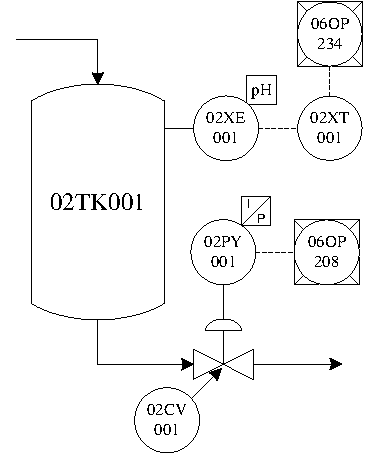
\includegraphics[width = 0.45\textwidth]{docupid}
		\caption{Cable marking}
		\label{fig:docu:examp}
	\end{figure}

	The I/P converter and pH sensor have individual identification blocks denoting the conversion and measurement of 		the different instrumentation.
\end{example}

\section{Loop diagrams}
The wiring system has many connections that must be documented in an efficient unambiguous way. The standard format used for the documentation of analog and digital control loops are \eindex{loop diagrams}\citep[143]{Mulley93}. An example of the loop diagram for the two control valves of the pH control loop in the control laboratory can be seen in figure~\ref{fig:wire:wired}.
\begin{sidewaysfigure}[p]
	\centering
	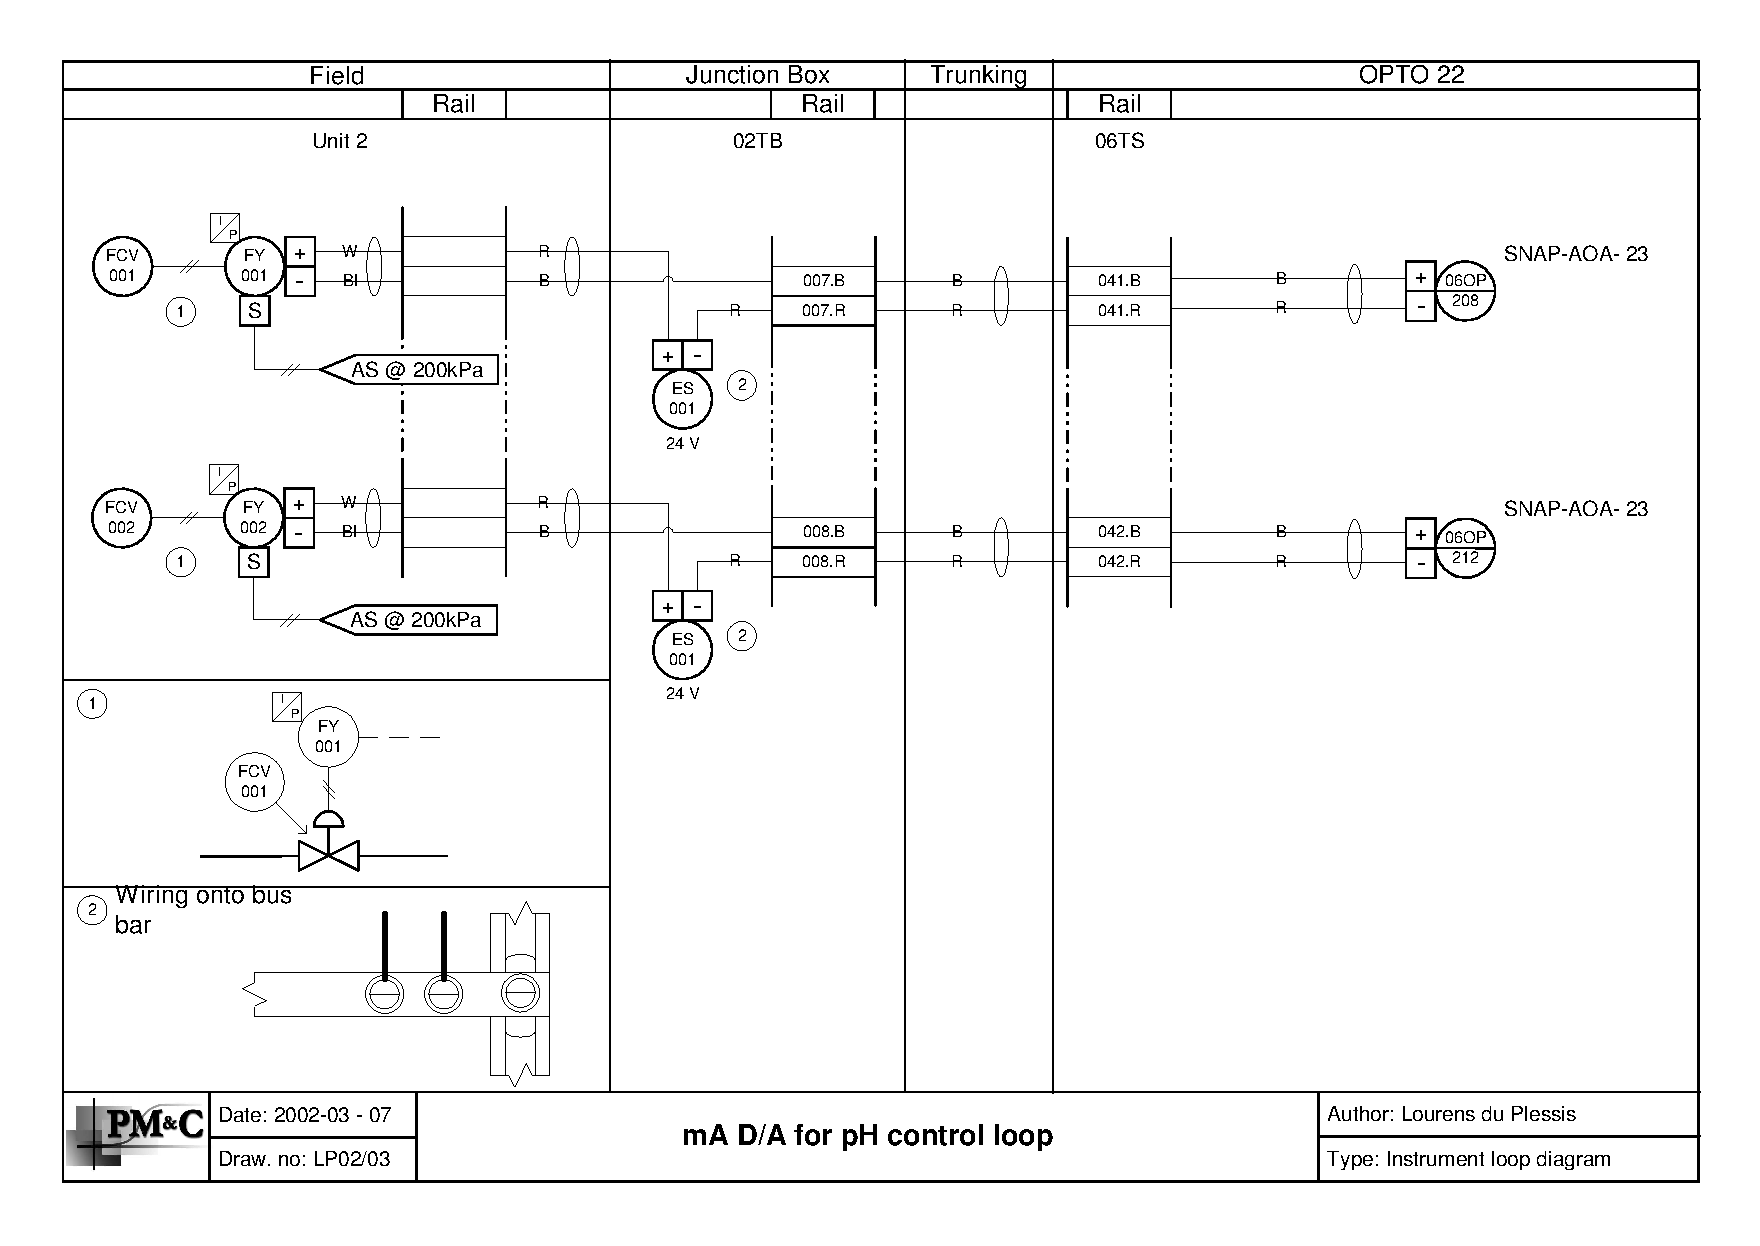
\includegraphics[width = \textwidth]{wirewired}
	\caption{Wire diagram of the control valves of the pH control loop}
	\label{fig:wire:wired}
\end{sidewaysfigure}

It can be seen that the electrical wiring of the system is shown with the associated instrumentation of the loop. The diagram will therefore greatly assist in the detection and correction of faults or the installation of new instrumentation. The diagram consist further out of four main areas, separated by vertical lines the definition of these areas follows.
\begin{description}
	\item[Field] defines the instrumentation on the experimental setup. The instrumentation usually associated with the field are are sensors, actuators, converters and transmitters.
	\item[Junction box] defines the wiring inside the junction box. The power supply and connectors with their corresponding identification number or tag are clearly shown. It should be noted however that the full connector number consist out of the number shown on the connector as well as the rail number. The tag number for the connector is therefore 02TBXXX.C with the C denoting either the red (R) or blue (B) wire.
	\item[Trunking] is the wiring between the \eindex{junction box} and the \eindex{Opto box}.
	\item[OPTO22] is the instrumentation inside the \eindex{Opto box}. The connectors are again shown with the \eindex{SNAP modules}. The Opto box is allocated unit number six 06, the connector tag number will therefore be 06TSXXX.C. The two opto racks are defined by numbers 1 and 2. The tag number for a specific measurement will therefore be 06OP1XX or 06OP2XX depending on the associated rack of the current model.  
\end{description}

\section{Tag number marking}
\subsection{Cable marking}
The numbering of the different cables are affixed to the cable using specific colour coded cable markers. The cable number contains two parts, the connector number from the cable origin and the connector number of the destination connector. 

The cable number is affixed on both ends of the cable. The exact source and  origin of the cable can accordingly be seen at any end; reducing the effort for maintenance and fault detection. The connectors are marked as well using smaller plastic numbering clips with the same colour scheme as that used for the cables. 

The direction of the numbering is always from the \eindex{experimental setup} to the \eindex{Opto box} with a dash separating the two numbers.  An example can be seen in figure~\ref{fig:wire:mark2} with the tag numbering flow from the experimental setup (001) to the Opto box (201), which is in this case from left to right.
\begin{figure}[htbp]
	\centering
	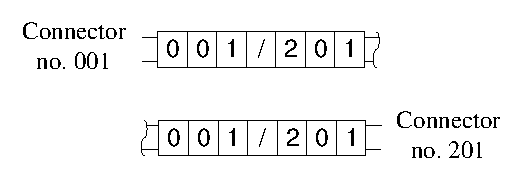
\includegraphics[width = 0.5\textwidth]{wiremark2}
	\caption{Cable marking}
	\label{fig:wire:mark2}
\end{figure}

\subsection{Instrument marking}
The instrumentation is marked clearly with a tag defining the full tag number of the instrument. ``Cable ties'' are used to fix the marker onto the instrumentation (see figure~\ref{fig:wire:valvemark}).
\begin{figure}[htbp]
	\centering
	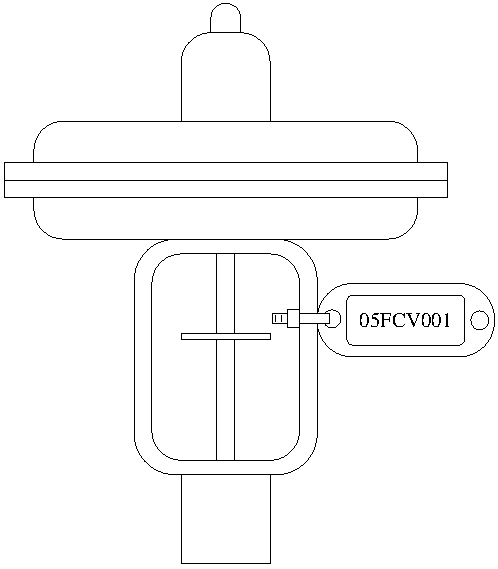
\includegraphics[width = 0.4\textwidth]{wirevalvemark}
	\caption{Instrument marking}
	\label{fig:wire:valvemark}
\end{figure}

\section{Equipment Database}
To simplify the documentation of the wiring and connectors, an \eindex{equipment database} is required. This database tracks each piece of process control equipment and the connections between them. The database can be obtained at $\backslash$$\backslash$groa$\backslash$phpMyAdmin.

The starting point for the database is the rig table, which contains the number and name of all the experimental setups.  From here, linked to the rig number an equipment table stores each item's type and number.  In addition, data is stored about the date of acquisition and origin of the equipment to simplify maintenance and reordering.  To make the database expendable, a table of equipment types is linked to the equipment table, storing the tag extension of the equipment type. 

Queries are defined to generate tag numbers in accordance with the standards set out above, by combining the rig number, equipment type extension and the equipment number.

In order to track connections, each equipment record also stores the unique ID of another piece of equipment.  The direction of this linked list is defined as away from the final control elements and measuring devices.  Therefore, a control valve will link to the \eindex{junction box} connector and an OPTO SNAP analog in module will link to the \eindex{junction box} connector.  

Wire names are generated by a \eindex{SQL query}, adding the numbers from the connected pieces of equipment.  A list of wire names can be drawn up in a report for wire checking. 

To keep the documentation current, the following steps are required when adding new equipment.
\begin{description}
\item[Step 1] Collect information
The following information is pertinent when installing new equipment:
\begin{itemize}
	\item	What type of signal does the equipment send or receive?  This will determine the module on the OPTO that the equipment will be wired to.
	\item	Are there enough connectors in the \emph{junction box} to accommodate the new signal?  If not, new connectors must be installed.
	\item	Are there enough OPTO modules of the type required? If not, a new OPTO module must be installed.
\end{itemize}

\item[Step 2] Add the equipment to the equipment database.
Check that the equipment type exist by double clicking the equipment type table.  If the equipment type does not exist, add a new type on the last line of the table and close the table view.  Open the equipment table by double clicking it.  Select the rig and equipment type from the drop down list.  Enter a unique number for the equipment in the number field, then select the tag number of the equipment this item is connected to.  For instance, a thermocouple would be connected to a connector in the \eindex{junction box} for the experimental setup. If there are no free connectors in the \eindex{junction box}, follow the same steps as above for two new connectors: one in the \eindex{junction box} and one in the \eindex{Opto box}.

\item[Step 3] Lay the wiring
Open the trunking and lay a new wire between the \emph{Opto box} and the \emph{junction box}, bearing in mind that the wire must be labelled with its wire number.  Use the wire number for the wire between the connectors mentioned above.  This number is generated automatically by the database in the wire numbers query.

\item[Step 4] Connect the wires
The wires are now connected between connectors.

\item[Step 5] Test
Before the equipment is used, a signal check must be run.  Using a Ohmmeter, check the resistance between the terminals of the new signal.  This should be very high.  Low values indicate a short circuit.

\item[Step 6] Connect equipment and OPTO
The wires are now connected to the equipment and to the OPTO module.
\end{description}

An example of the database interface can be seen in figure~\ref{fig:docu:interface} and shows the different experimental setups of the process control laboratory.
\begin{figure}[htbp]
	\centering
	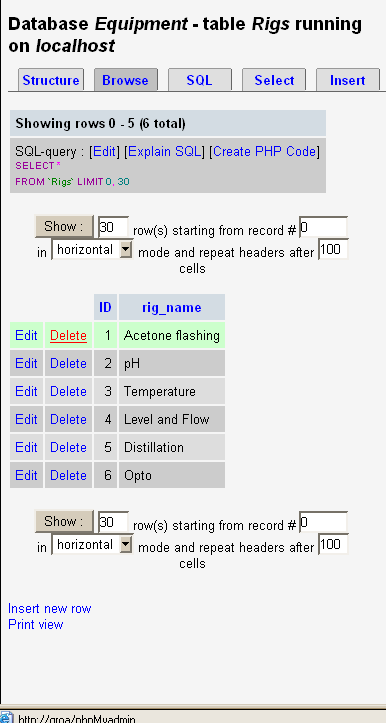
\includegraphics[width = 0.6\textwidth]{interface}
	\caption{Equipment database interface}
	\label{fig:docu:interface}
\end{figure}
\chapter{Tips}

This chapter will contain tips related to different types of software and hardware issues in the lab.

\section{Matlab}

\section{Aspen}

\section{Hardware}

\appendix

\chapter{Wiring nomenclature tables}

The following tables are relevant for the tagging and labeling of lab equipment:

\begin{table}[H]
\centering
\caption[Rig numbers]{Lab wiring - Rig numbers}
\begin{tabular}{ll}
Number & 	Setup name \\
\hline
01 & Acetone flashing \\
02 & pH \\
03 & Temperature \\
04 & Level and flow \\
05 & Distillation \\
06 & OPTO22 setup \\
\end{tabular}
\end{table}

\begin{table}[H]
\centering
\caption[Object types]{Object types for tag numbers}
\begin{tabular}{ll}
Object & Tag code \\
\hline
Control Valve & CV \\
Setup JB connector & TB \\
OPTO22 JB connector	& TS \\
Differential pressure cell & DP \\
Thermocouple & TE \\ 
Level indicator	& LI \\
Thyristor & TC \\
\end{tabular}
\end{table}




\bibliographystyle{chemeng}
\bibliography{lab}

\printindex

\end{document}